% Options for packages loaded elsewhere
\PassOptionsToPackage{unicode}{hyperref}
\PassOptionsToPackage{hyphens}{url}
%
\documentclass[
]{article}
\usepackage{amsmath,amssymb}
\usepackage{iftex}
\ifPDFTeX
  \usepackage[T1]{fontenc}
  \usepackage[utf8]{inputenc}
  \usepackage{textcomp} % provide euro and other symbols
\else % if luatex or xetex
  \usepackage{unicode-math} % this also loads fontspec
  \defaultfontfeatures{Scale=MatchLowercase}
  \defaultfontfeatures[\rmfamily]{Ligatures=TeX,Scale=1}
\fi
\usepackage{lmodern}
\ifPDFTeX\else
  % xetex/luatex font selection
\fi
% Use upquote if available, for straight quotes in verbatim environments
\IfFileExists{upquote.sty}{\usepackage{upquote}}{}
\IfFileExists{microtype.sty}{% use microtype if available
  \usepackage[]{microtype}
  \UseMicrotypeSet[protrusion]{basicmath} % disable protrusion for tt fonts
}{}
\makeatletter
\@ifundefined{KOMAClassName}{% if non-KOMA class
  \IfFileExists{parskip.sty}{%
    \usepackage{parskip}
  }{% else
    \setlength{\parindent}{0pt}
    \setlength{\parskip}{6pt plus 2pt minus 1pt}}
}{% if KOMA class
  \KOMAoptions{parskip=half}}
\makeatother
\usepackage{xcolor}
\usepackage{longtable,booktabs,array}
\usepackage{calc} % for calculating minipage widths
% Correct order of tables after \paragraph or \subparagraph
\usepackage{etoolbox}
\makeatletter
\patchcmd\longtable{\par}{\if@noskipsec\mbox{}\fi\par}{}{}
\makeatother
% Allow footnotes in longtable head/foot
\IfFileExists{footnotehyper.sty}{\usepackage{footnotehyper}}{\usepackage{footnote}}
\makesavenoteenv{longtable}
\usepackage{graphicx}
\makeatletter
\def\maxwidth{\ifdim\Gin@nat@width>\linewidth\linewidth\else\Gin@nat@width\fi}
\def\maxheight{\ifdim\Gin@nat@height>\textheight\textheight\else\Gin@nat@height\fi}
\makeatother
% Scale images if necessary, so that they will not overflow the page
% margins by default, and it is still possible to overwrite the defaults
% using explicit options in \includegraphics[width, height, ...]{}
\setkeys{Gin}{width=\maxwidth,height=\maxheight,keepaspectratio}
% Set default figure placement to htbp
\makeatletter
\def\fps@figure{htbp}
\makeatother
\setlength{\emergencystretch}{3em} % prevent overfull lines
\providecommand{\tightlist}{%
  \setlength{\itemsep}{0pt}\setlength{\parskip}{0pt}}
\setcounter{secnumdepth}{-\maxdimen} % remove section numbering
\ifLuaTeX
  \usepackage{selnolig}  % disable illegal ligatures
\fi
\IfFileExists{bookmark.sty}{\usepackage{bookmark}}{\usepackage{hyperref}}
\IfFileExists{xurl.sty}{\usepackage{xurl}}{} % add URL line breaks if available
\urlstyle{same}
\hypersetup{
  pdftitle={A Fast GPU Algorithm for Carving Simulation},
  hidelinks,
  pdfcreator={LaTeX via pandoc}}

\title{A Fast GPU Algorithm for Carving Simulation}
\author{}
\date{}


%% ---- rev3 additions (clean-up of pandoc output) ----
\usepackage[margin=1in]{geometry}
\ifPDFTeX
\usepackage{newunicodechar}
% Only symbols NOT already defined by the LaTeX kernel's utf8 support
% (recent TeX Live); the predefined ones are left to the kernel to avoid warnings.
\newunicodechar{≈}{\ensuremath{\approx}}
\newunicodechar{Δ}{\ensuremath{\Delta}}
\newunicodechar{≤}{\ensuremath{\leq}}
\newunicodechar{≥}{\ensuremath{\geq}}
\newunicodechar{⌈}{\ensuremath{\lceil}}
\newunicodechar{⌉}{\ensuremath{\rceil}}
\newunicodechar{√}{\ensuremath{\surd}}
\newunicodechar{∪}{\ensuremath{\cup}}
\newunicodechar{−}{\ensuremath{-}}
\newunicodechar{∈}{\ensuremath{\in}}
\newunicodechar{∞}{\ensuremath{\infty}}
\newunicodechar{≫}{\ensuremath{\gg}}
\newunicodechar{↔}{\ensuremath{\leftrightarrow}}
\newunicodechar{⇒}{\ensuremath{\Rightarrow}}
\newunicodechar{⊕}{\ensuremath{\oplus}}
\newunicodechar{Σ}{\ensuremath{\Sigma}}
\newunicodechar{₁}{\textsubscript{1}}
\newunicodechar{₂}{\textsubscript{2}}
\newunicodechar{ₙ}{\textsubscript{n}}
\fi
\setcounter{secnumdepth}{0} %% headings carry their own manual numbers
\setlength{\emergencystretch}{3em} %% relax line breaking (avoid overfull boxes)
\setlength{\tabcolsep}{3pt}
%% -----------------------------------------------------
\begin{document}
\begin{center}
{\LARGE\bfseries A Fast GPU Algorithm for Carving Simulation}\par
\end{center}
\bigskip


Nicola Scuor¹*, Philip Long², Stefano Seriani¹, Paolo Gallina¹

¹ Department of Engineering and Architecture, University of Trieste, Via
Alfonso Valerio 6/1, 34127 Trieste, Italy

² Department of Electronic, Software and Advanced Manufacturing
Engineering, Atlantic Technological University, Galway, Ireland

* Corresponding author: Nicola Scuor,
\href{mailto:nscuor@units.it}{\nolinkurl{nscuor@units.it}}

ORCID

Nicola Scuor: 0000-0002-5073-637X

Philip Long: 0000-0002-0784-8720

Stefano Seriani: 0000-0002-5563-9595

Paolo Gallina: {[}to be inserted{]}

\hypertarget{abstract}{%
\subsection{Abstract}\label{abstract}}

Material-removal (carving) simulation, i.e. computing the workpiece geometry
that a milling program actually produces, is a core primitive of
computer-aided manufacturing: toolpath verification, cutting-force and
cutter-workpiece engagement estimation, machining digital twins, and
process- or toolpath-optimization and learning loops all rely on it, and
call it repeatedly, from many times in an interactive check to millions
inside a search, so its throughput sets the scale of study that is
feasible at all \textcolor{red}{[10-15]}. We present a GPU algorithm for this
simulation that is, to the best of our knowledge, the fastest reported
for dexel-based milling material removal. It is built on a single-axis
dexel field, a grid of columns storing sorted height transitions, in
which Boolean subtraction becomes an independent per-column merge that
maps one workpiece column to one GPU thread. Against two established
baselines, per-step stamping and swept-volume subtraction through a
separate buffer, we contribute two optimizations. Fused swept-segment
subtraction computes each move\textquotesingle s swept extent on the fly
as a per-column envelope and subtracts it in place, never materializing
the swept volume; it is 1.85 times faster than the external-buffer
baseline and halves resident memory. Tube pruning skips the write-back
for dispatched columns the tool never touches, giving 3.2 to 7.4 times
on diagonal and air-heavy programs, at up to 8\% cost on dense
axis-aligned rasters. Two negative results and one positive one support
a single diagnosis: the levers that pay remove memory-write traffic, not
arithmetic or launched threads: the simulation is bound by write
bandwidth to the working-set buffer. Every optimization level is
byte-identical, and exact against an analytic reference on axis-aligned
moves. The method is a drop-in accelerator for the many CAM workflows
bottlenecked by repeated carving simulation.

\textbf{Keywords:} Material-removal simulation, GPU compute, Dexel
model, Swept volume, Machining simulation, CAM

\hypertarget{introduction}{%
\subsection{1. Introduction}\label{introduction}}

\hypertarget{motivation}{%
\subsubsection{1.1 Motivation}\label{motivation}}

Material-removal simulation predicts the workpiece geometry a milling
program produces by repeatedly subtracting the cutting
tool\textquotesingle s swept volume from a stock model. It is a
workhorse of computer-aided manufacturing: it underlies toolpath
verification and gouge or collision checking \textcolor{red}{[15]}, cutting-force and
cutter-workpiece engagement estimation \textcolor{red}{[10, 11]}, machining digital
twins \textcolor{red}{[12]}, and -increasingly- optimization \textcolor{red}{[13]} and learning
\textcolor{red}{[14]} loops that search over candidate toolpaths and score each
against a target. In all of these the simulator is called repeatedly,
from many times in an interactive verifier to millions inside a search
or a training run, so its raw throughput at a fixed, adequate accuracy
sets the scale of study that is feasible at all. A fast and accurate
forward model, i.e. one that, given a toolpath, tool and stock, computes the
resulting workpiece - is therefore the enabling primitive, and it is the
object of this paper.

Raw simulation speed at a fixed, adequate accuracy is thus the central
requirement and the primary driver of the design choices below; the
method\textquotesingle s geometric error against the continuously-swept
cut is zero on axis-aligned moves and 0.08 \% on diagonals, measured
against an analytic reference in §4.6, so accuracy here is a constraint
to hold, not the quantity we optimize. We restrict the scope to milling
in which the tool translates with its axis fixed to Z (three-axis
machining) and to programs of linear moves, G00 and G01; circular
interpolation is handled upstream by rendering arcs as polylines, and
each resulting segment is the input the method takes.

\hypertarget{related-work}{%
\subsubsection{1.2 Related work}\label{related-work}}

Column-based material-removal simulation begins with the dexel model
{[}1{]}, which renders NC milling in real time as an image-space Boolean
subtraction: the workpiece is a grid of Z-direction ``depth elements''
(dexels), and the tool lowers their heights. The model was extended to
multi-/tri-dexel representations (three orthogonal dexel bundles) to
improve sampling on steep walls: {[}2{]} present online sculpting on
multi-dexel volumes, and GPU variants were developed {[}3, 4{]}. In
parallel, the solid-modeling community proposed sparse, per-axis
implicit representations with GPU Booleans, notably Layered Depth-Normal
Images, LDNI {[}5{]}. Swept-volume computation has its own line, from
the sweep-envelope differential equation {[}6{]} to the survey {[}7{]}.
Surface reconstruction uses Marching Cubes {[}8{]}, and its
corresponding GPU version {[}9{]}.

Two observations frame what follows. First, subtracting a
tool\textquotesingle s swept volume per move from a dexel model is not
new; it is exactly what {[}2, 3, 4{]} do, and we treat it as a baseline
rather than a contribution. Second, that line of work optimizes the
geometry of the subtraction, while the cost we measure is dominated by
the traffic to the working-set buffer, a resource none of it addresses.
Our contribution is therefore not a new representation but a different
target.

\hypertarget{contributions}{%
\subsubsection{1.3 Contributions}\label{contributions}}

We present two optimizations, both implemented entirely on the GPU and
each isolated by A/B comparison against the best available baseline from
the literature. We label the four levels S0 to S3 throughout: per-step
stamping (S0), swept subtraction through an external buffer (S1), the
fused in-place swept kernel (S2), and the fused kernel with tube pruning
(S3); the first two are the established baselines and the last two are
this work, and §6.1 anchors each to the literature it represents. Each
of ours is byte-identical to the swept baseline it builds on, S0 being a
timing and behavioural reference rather than a geometric ground truth
(§4.6).

\textbf{Contribution 1: Fused swept-segment subtraction.} For each
linear toolpath segment, the swept-tool column is computed on the fly as
a Z-envelope and subtracted in place, never materializing the swept
volume. Because columns are independent, the operation maps directly to
one GPU thread per column. Compared to an external-buffer swept baseline
(which writes the swept volume to a separate buffer and subtracts it in
a second pass), fusion is ≈1.2--2.5× faster (geomean ≈1.85×) and halves
resident memory: the external buffer requires a full-size twin of the
working set that the fused kernel eliminates (§6.1, §6.3). This is a
consistent win across all workloads.

\textbf{Contribution 2: Tube pruning with in-air skip.} The GPU dispatch
covers the axis-aligned bounding box of each segment\textquotesingle s
endpoints, which on diagonal moves and in-air rapids is far larger than
the actual swept band. We skip the per-column write-back for columns the
tool never touches, leaving them untouched and the result
byte-identical. Tube pruning delivers 3.2--7.4× on the stress benchmarks
(Table 1), while staying neutral-to-modest-cost on axis-aligned programs
(at most ≈8 \% on the densest raster, where the dispatch already matches
the swept band, §6).

Beyond these two main contributions, we introduce three additional
refinements that improve specific aspects of the method. First, we
perform GPU-side result compaction, which reduces read-back traffic by
approximately an order of magnitude by returning only the compact
transition lists rather than the full unpacked buffer (§3.5). Second, we
implement a sparse tiled backend that materializes only the tiles
actually touched during carving. This is a memory/scale lever rather
than a speed optimization: for localized programs, it shrinks the
resident footprint to a small fraction of the full buffer; for
whole-stock machining, however, it offers no saving. The backend is
runtime-selectable and byte-identical to the flat buffer version (§6.2).
Third, we eliminate the dead trailing zero-fill of each column's
write-back: byte-identical, it removes write traffic on the active
columns for 8--22\% on the fused kernel, reaching the axis-aligned case
where tube pruning does not (§6.4).

We also report two attempted optimizations that we implemented in full
and then discarded because they did not pay off. The first was a
range-query envelope acceleration: we precomputed per-tool directional
Z-envelopes as sparse tables, turning the per-column envelope
computation from an O(sub-steps) loop into an O(1) query. This gave only
modest improvement, because it optimized compute, which is not the
bottleneck, and was reverted. The second was an oriented tiled dispatch:
we attempted to tile the launch along the swept band itself, so that
off-band threads would not even be launched. This required barriers
between tiles to preserve byte-identity, and the resulting
synchronization overhead, together with overlapping joins between
adjacent tiles, made the approach slower than tube pruning alone. We
reverted it as well. Together, these negative results corroborate our
central diagnosis: on this pipeline, the lever that pays is the one that
removes memory-write traffic, not the ones that reduce compute or
launched threads (§7).

\hypertarget{volume-representation-single-axis-dexel-field}{%
\subsection{2. Volume representation: single-axis dexel
field}\label{volume-representation-single-axis-dexel-field}}

Both the stock and the tool are discretised on a common voxel lattice of
W × H × D cells, but that lattice is never materialised: it only fixes
the sampling resolution and the integer coordinates in which every
quantity is expressed. What is actually stored is a single-axis dexel
field along Z. Each (x, y) column of the lattice is a one-dimensional
occupancy function of z, encoded as the sorted list of the heights at
which occupancy flips: empty to solid or solid to empty. Because
occupancy alternates, transitions come in pairs, one entering and one
leaving the solid (Fig. 1).

Milling parts are massive bodies bounded by a few surfaces, so a column
crosses the boundary only a handful of times: two to four transitions is
typical, and two is the minimum, since transitions come in pairs. An
uncarved column of a prismatic stock is exactly that minimum, the single
pair {[}0, z\_top{]}, where z\_top is the height of the
stock\textquotesingle s top face: solid from the base up to that face,
empty above. For a stock that fills the lattice, z\_top coincides with
the grid depth z1 used as the clamping bound in §3.6 and §4.4.

\begin{center}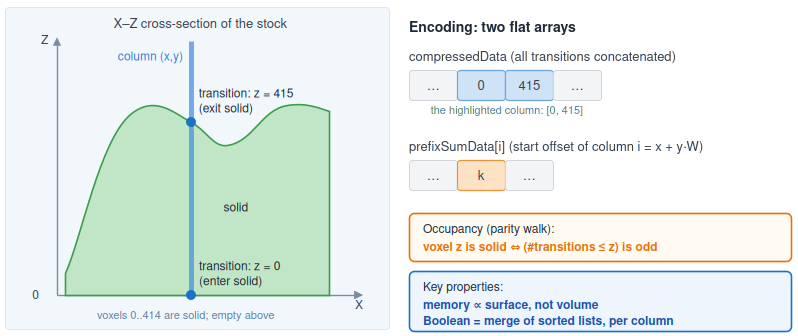
\includegraphics[width=6.26806in,height=2.63889in]{figures/image1.png}\end{center}

\textbf{Fig.
1} The single-axis dexel (Z-transition column) representation. A column
stores the sorted heights at which occupancy flips; two flat arrays
encode the whole object, and occupancy at any voxel is recovered by a
parity walk. Storage scales with the complexity of the boundary rather
than with the enclosed volume, and any Boolean operation becomes a merge
of sorted lists, independent per column

The whole object is a struct VoxelObject, used for both stock and tool,
consisting of two flat arrays. Columns are addressed by the linear index
i=x+y*W, i.e.~row-major with X varying fastest, and both arrays follow
that order:

\begin{itemize}
\item
  compressedData: the transition lists of all columns, each sorted
  ascending, concatenated in order of i.
\item
  prefixSumData: for each column i, the offset at which its list begins
  in compressedData. The array has one entry per column, so the length
  of column i's list is prefixSumData{[}i+1{]} − prefixSumData{[}i{]},
  with the last column running to the end of compressedData. During a
  carving session the resident stock keeps its per-column counts in a
  separate array instead (§4.2).
\end{itemize}

The name is historical: the struct stores transitions, not voxels.

Occupancy at (x, y, z) is recovered by a parity walk: the voxel is solid
iff the number of transitions of its column that are ≤ z is odd. No
dense buffer is ever allocated, read or written.

Three properties are exploited throughout.

\begin{enumerate}
\def\labelenumi{\arabic{enumi}.}
\tightlist
\item
  Compactness: storage is proportional to the number of transitions,
  that is, to how often the columns cross the boundary, and not to the
  enclosed volume. A field averaging c transitions per column costs
  c*W*H integers where a dense grid would cost W*H*D occupancy values, a
  saving of a factor D/c.~For c ≈ 2 to 4 and the depths typical of a
  milling stock this is two to three orders of magnitude, and it does
  not grow as the part becomes more massive, only as its surface becomes
  more intricate (absolute figures for the reference stock of §5.2 are
  given in §6.3).
\end{enumerate}

\begin{enumerate}
\def\labelenumi{\arabic{enumi}.}
\tightlist
\item
  Boolean = per-column merge. Any Boolean between two fields on the same
  lattice is a two-pointer merge of their sorted transition lists,
  performed independently for each of the W*H columns: the traversal is
  the same in every case, only the predicate on the two occupancy states
  differs (AND for intersection, OR for union, AND-NOT for difference),
  and a transition is emitted wherever the predicate changes value. The
  carver uses difference alone (subtracting the tool from the stock) and
  it is the only operation implemented on the GPU (§4.4). Columns never
  interact, so the merge is embarrassingly parallel and maps to one GPU
  thread per column (§4.1).
\item
  A free bounding interval. The lowest and highest transitions of a
  column are exactly its solid extent {[}bottom, top{]}, available
  without a search. For tools whose columns are a single Z-interval
  (§4.5) that interval is not a bound on the column: it is the column;
  this makes the on-the-fly Z-envelope of §3.3 possible.
\end{enumerate}

\hypertarget{from-naive-stamping-to-the-final-solution}{%
\subsection{3. From naive stamping to the final
solution}\label{from-naive-stamping-to-the-final-solution}}

We build the method as a sequence of refinement levels, each validated
against the previous one (byte-identical among the swept levels; §4.6).
To make the transformations concrete we follow one setting throughout: a
prismatic stock, a ball-end mill, that is, a cylinder closed by a
hemispherical tip of the same radius, and a single linear segment
carrying the tool from p0 to p1. No dimensions are needed here, since
none of the steps depends on them; the measured configurations are those
of §5.

The tool is positioned by the centre of its own bounding box: the G-code
coordinate, converted to voxel units, places that centre, with no
compensation for the tip radius or the shank length. This is a
calibration convention rather than a modelling choice, and it applies
identically to every refinement level, so it affects none of the
comparisons below. It does mean that a real G-code program in
millimetres cannot yet be consumed without an external calibration step
(§7).

\hypertarget{naive-stamping-baseline}{%
\subsubsection{3.1 Naive stamping
(baseline)}\label{naive-stamping-baseline}}

The naive simulator advances the tool along the segment in fixed jog
steps and stamps the whole tool at each of them, one Boolean-difference
dispatch per step, subtracting the tool at that position from the stock.
The step s is a fixed distance in voxel units along the segment,
independent of the segment\textquotesingle s direction and length. A
segment of length L thus costs approximately L/s dispatches. This
approach has two sources of inefficiency. First, the dispatches overlap:
consecutive positions differ by s while the tool footprint is many
voxels wide, so every column under the tool is read, merged and
rewritten several times over, even though only the first of those passes
typically removes material. Second, the sampling is visible in the
result: between two stamps the tool is never evaluated, so for
s\textgreater1 the carved floor exhibits a stepped profile (Fig. 2a).
Because the stamper is a union of stamps, refining the step can only add
positions to that union, never remove any; its removed volume grows
monotonically as s shrinks, approaching the continuous cut from below in
removed volume. §4.6 discusses how the single-pass swept subtraction
relates to that limit and to the stamper.

\begin{center}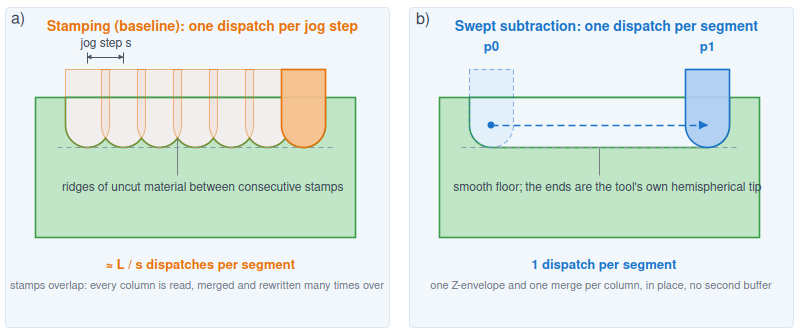
\includegraphics[width=6.26806in,height=2.60069in]{figures/image3.png}\end{center}

\textbf{Fig.
2} Stamping versus swept subtraction. Left: many overlapping stamps
along the path: a coarse step leaves a stepped floor and re-processes
each column many times (the tool is a ball-end mill: hemisphere tip plus
shank). Right: a single subtraction of the swept volume, one pass with a
step-free floor

\hypertarget{swept-segment-subtraction}{%
\subsubsection{3.2 Swept-segment
subtraction}\label{swept-segment-subtraction}}

Instead of L/s stamps we perform one subtraction per linear segment, of
the tool\textquotesingle s swept volume, i.e., the union of all tool
positions along the segment (Fig. 2b; formally, the Minkowski sum of the
tool geometry and the line segment; see {[}7{]} for a comprehensive
treatment). Set difference is order-independent and distributes over
unions, so subtracting the swept volume once equals stamping at every
sampled sub-position along the segment. This drastically reduces the
number of dispatches (quantified in §6, Table 2).

\hypertarget{on-the-fly-z-envelope-fused-in-one-kernel-core-contribution}{%
\subsubsection{3.3 On-the-fly Z-envelope, fused in one kernel (core
contribution)}\label{on-the-fly-z-envelope-fused-in-one-kernel-core-contribution}}

The subtlety is that "subtract the swept volume" appears to require
building that volume in a separate buffer and then subtracting it. We
never build it. The property that makes this possible is that each XY
column of the tool is a single solid interval in Z, from its lowest
point to its top. This holds for the standard 3-axis tool shapes:
ball-end, flat-end, conical and bull-nose cutters are all convex in Z,
and the shank that closes them from above does not break the property.
For the ball-end mill of our running example, the interval runs from the
hemisphere bottom up to the shank top. Tools that violate it are
discussed in §4.5.

Consider a fixed stock column. Only a contiguous range of sub-positions
along the segment actually overlaps that column; outside this range the
tool never covers it and the column stays unchanged. Within the range,
each sub-position contributes one interval, whose bottom depends on the
lateral offset between the tool axis and the column at that instant
(Fig. 3a). Since the tool advances by at most one voxel per sub-step,
the intervals contributed by consecutive sub-positions overlap; their
union is therefore again a single interval, {[}min bottom, max top{]},
which we call the Z-envelope (Fig. 3b). For a ball-end mill the deepest
bottom occurs at the sub-position where the tool axis passes closest to
the column, reaching the tip depth for a column that lies directly under
the path; for a flat-end cutter the bottom is the same at every covering
sub-position. The maximum top is the shank top, which lies above the
stock at every instant.

\begin{center}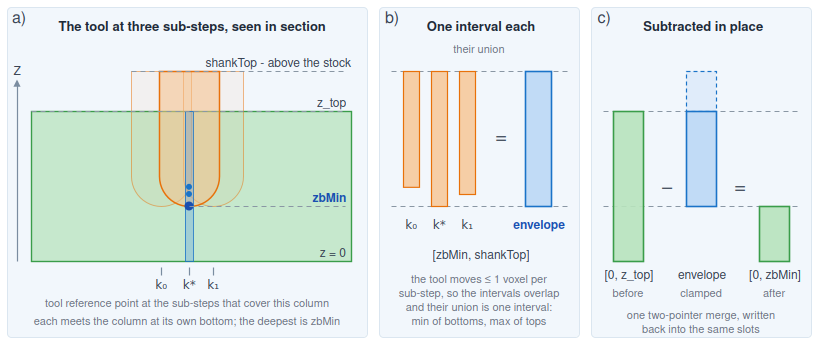
\includegraphics[width=5.83333in,height=2.44375in]{figures/image5.png}\end{center}



\textbf{Fig. 3} The per-column Z-envelope. The three panels share one
vertical Z scale. (a) Vertical section through the tool axis: the
ball-end mill at three sub-steps over one fixed stock column, with the
shank rising out of the workpiece. Each sub-step meets the column at its
own hemisphere bottom; the deepest occurs at the sub-step where the tool
passes closest to the column. (b) Each column of the tool is a single
interval in Z, so every sub-step contributes {[}bottom(k), shankTop{]}.
Because the tool moves by at most one voxel per sub-step, consecutive
intervals overlap and their union is again one interval: the envelope
{[}zbMin, shankTop{]}. (c) The envelope is subtracted from the column in
place, the shank-top transition being clamped away because it lies above
z\_top, leaving {[}0, zbMin{]}

A single fused compute shader accumulates this envelope in registers as
it walks only the sub-positions that overlap the column, then subtracts
it from the column in place, in the same pass (Fig. 3c): a two-pointer
merge of the stock column against one interval, with the shank-top
transition clamped away, since it lies above the stock surface. A column
that starts as {[}0, z\_top{]} ends as {[}0, zbMin{]}, exactly what
stamping at every sub-position of that range would produce (§4.6), from
a short loop and one merge, with no buffer for the swept volume. The
range of covering sub-positions is computed in closed form, as described
in §3.4.

§6.1 and §6.3 measure what this fusion buys against the external-buffer
version, which needs a second full buffer and an extra pass.

\hypertarget{sub-step-bounding}{%
\subsubsection{3.4 Sub-step bounding}\label{sub-step-bounding}}

The range of sub-positions that actually cover a given column, {[}k0,
k1{]}, can be computed directly from the segment geometry without
iterating over all sub-steps. For a linear toolpath segment from p0 to
p1, the tool centre moves along a straight line in the XY plane. The
tool is a solid of revolution about Z, so its XY footprint is a square
of side F voxels and its radius is F/2. The lateral distance between the
tool axis and a fixed column (x, y) is a convex quadratic function of
the interpolation parameter t ∈ {[}0, 1{]}; the times at which this
distance equals F/2 define the boundaries of the covering interval. The
enclosing range {[}k0, k1{]} in sub-step indices is then obtained by
projecting the column onto the segment, clamping to the segment
endpoints, and dilating by F/2. A small safety margin (±1 voxel) is
added to account for numerical rounding and to ensure that no covering
sub-position is missed. Iterating only this range per column reduces the
per-column work from the full segment length to approximately the tool
extent on axis-aligned moves, and to a similarly reduced band on
diagonal moves.

\hypertarget{gpu-compaction-for-read-back}{%
\subsubsection{3.5 GPU compaction for
read-back}\label{gpu-compaction-for-read-back}}

After carving, the result must be returned to the host in the compact
column format. Reading back the unpacked working buffer would transfer
the entire fixed-stride flat buffer, including all unused slots, which
is wasteful. Instead, we compact the result on the GPU first (§4.2),
producing a densely packed transition list that contains only the actual
transitions of each column. This reduces the read-back traffic by
approximately an order of magnitude, since the compact representation
transfers only the transitions that are actually present, rather than
the full allocated buffer. Quantitative figures for the reference
benchmark are given in §6.3.

\hypertarget{tube-pruning-the-new-optimization}{%
\subsubsection{3.6 Tube pruning (the new
optimization)}\label{tube-pruning-the-new-optimization}}

The dispatch (§4.3) covers the axis-aligned bounding box (AABB) of the
two tool-centre endpoints, dilated by the tool footprint (Fig. 4a). For
an axis-aligned move, that AABB already equals the swept band, but for a
diagonal move of length L it is approximately (0.7L+F)\^{}2 columns
while the tool sweeps only approximately L*F, so most of the dispatch
falls outside the band. Every over-covered column still rewrites its
entire allocated slot count for a no-op, because the shader had no
early-out before its write-back (Fig. 4b). In-air rapid (G0) moves are
the same: the tool is above the stock, so every column is a no-op that
still rewrites its slots (Fig. 4c).

\begin{center}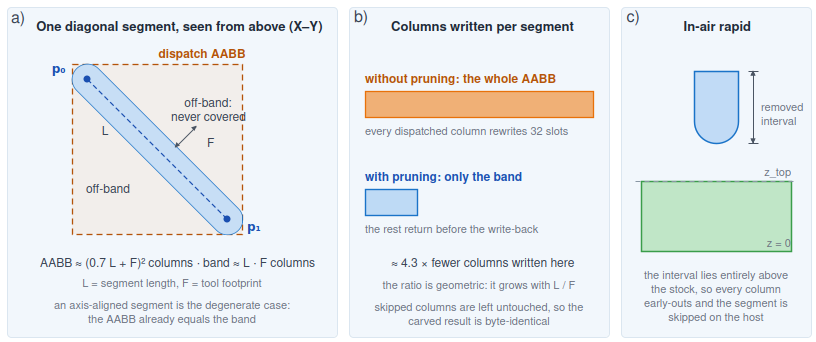
\includegraphics[width=5.83333in,height=2.44375in]{figures/image7.png}\end{center}



\textbf{Fig. 4} Tube pruning. (a) A long diagonal segment seen from
above: the dispatch AABB (dashed) is far larger than the swept band it
contains, and the off-band columns are no-ops that the baseline still
rewrites. (b) Columns written per segment, with and without pruning, in
the ratio given by the geometry drawn in (a); skipping the write-back
leaves the off-band columns untouched, so the result is byte-identical.
(c) In-air rapids are the extreme case: the removed interval lies
entirely outside the stock\textquotesingle s Z-range, so every column is
skipped and the whole segment is dropped on the host. Panels (a) and (c)
correspond to the two branches of the same early-out

The solution is a single early-out in the shader (§4.4): before the
merge and write-back, the shader returns when the tool never covers the
column, which is the case of Fig. 4a, or when the removed interval lies
entirely outside the stock\textquotesingle s Z-range, the case of Fig.
4c. The column is left untouched, which is correct because it is
unchanged, and its write traffic vanishes. This is what makes
over-dispatched diagonals and in-air rapids cheap; axis-aligned
dispatches are fully covered, so the test never pays there and costs up
to 11\% (§6.1).

The same pruning applies one level up, on the host, at segment
granularity: when the tool\textquotesingle s Z-extent over a whole
segment cannot reach the stock\textquotesingle s {[}0, z1) range (the
common case for an in-air G0 rapid, which maps below the stock under the
inverted-Z convention), the segment removes nothing and its entire
dispatch is skipped, not merely pruned per column. Rapids become much
cheaper (quantified in §6, Table 1), and every program with
repositioning moves speeds up; this optimization is host-side,
byte-identical, and gated by the same toggle.

\hypertarget{algorithm-and-gpu-implementation}{%
\subsection{4. Algorithm and GPU
implementation}\label{algorithm-and-gpu-implementation}}

\hypertarget{a-short-gpu-compute-primer}{%
\subsubsection{4.1 A short GPU-compute
primer}\label{a-short-gpu-compute-primer}}

The pipeline uses compute shaders: programs that run on the GPU outside
the graphics pipeline. A program is launched by a dispatch that creates
a grid of workgroups; each workgroup contains a fixed block of threads
that execute the shader in parallel (in our case, local\_size = 8×8×1,
so 64 threads per workgroup). Each thread reads its
gl\_\allowbreak GlobalInvocationID, a three-dimensional index identifying it within
the whole grid. Data is stored in Shader Storage Buffer Objects (SSBOs):
large GPU-resident arrays that the shader reads and writes. Ordering
between dependent dispatches is enforced by a memory barrier. In our
carver, one thread processes one workpiece column; this is how the
per-column-merge property of the dexel representation (§2) maps directly
onto the hardware.

\hypertarget{data-layout-the-flat-working-buffer}{%
\subsubsection{4.2 Data layout: the flat working
buffer}\label{data-layout-the-flat-working-buffer}}

During a carving session the stock is held GPU-resident in a
fixed-stride flat buffer, obj1\_flat, of W*H*MAX\_TRANSITIONS unsigned
integers, plus a per-column count buffer obj1\_dataNum. Column (x, y)
owns the slice of MAX\_TRANSITIONS slots at offset
(x+y*W)*MAX\_TRANSITIONS. Subtractions write results in place into the
same slots, so no per-operation reallocation is needed. This buffer is
the working set whose bandwidth dominates the cost of a carve (§7); its
size for the reference stock of §5.2 is given in §6.3.

The value MAX\_TRANSITIONS = 32 is chosen as a safe upper bound. A
column crosses the boundary only a handful of times (§2), and even
complex parts rarely exceed a few dozen transitions, so a fixed stride
of 32 slots covers the vast majority of practical cases while keeping
memory access patterns regular and predictable. Occupancy queries read
only the first \texttt{obj1\_dataNum{[}i{]}} slots of a column, but the
write-back covers the whole stride: the merge writes the new transitions
and then zeroes the remaining slots. Every column the shader does not
skip therefore costs a full stride of write traffic, which is what the
early-out of §3.6 avoids and what §6.4 measures directly.

The stride is not overflow-guarded. If a column would produce more than
MAX\_TRANSITIONS transitions the merge stops there, the surplus is
dropped, and the truncated list is written back with its count; the
failure is a localised loss of geometry in that column, silent and
non-propagating, with the rest of the carve unaffected (§7). The margin
is generous, but a column needing more than MAX\_TRANSITIONS transitions
would be clipped rather than detected. We did not implement detection
because none of the geometries we target approaches the bound, and
inputs at that extreme are outside the scope of this work; it would be
near-free to add, since the merge loop already tests the stride bound at
every iteration and a flag would cost one atomic write on a branch that
is never taken in normal operation.

The tool is uploaded once as a compact (compressedData, prefixSumData)
pair and never mutates.

\hypertarget{dispatch-mapping-threads-onto-the-xy-grid}{%
\subsubsection{4.3 Dispatch: mapping threads onto the XY
grid}\label{dispatch-mapping-threads-onto-the-xy-grid}}

For each segment the host computes the swept bounding box, i.e.~the AABB
of the two tool-centre endpoints dilated by the tool half-footprint F/2,
then clamps it so that it addresses only columns in {[}0, W) × {[}0, H),
since a segment near an edge of the stock, or one passing outside it
altogether, would otherwise dilate past the grid. This gives an origin
(baseX, baseY) and a size (bboxW, bboxH) that address existing columns
only (Fig. 5a). The implementation reads the two tool extents (w2/2,
h2/2) separately only because the same structure also holds the
non-square stock. It then dispatches ⌈bboxW/8⌉ × ⌈bboxH/8⌉ workgroups
(Fig. 5b), and inside the shader each thread recovers its column as gx =
baseX+gl\_\allowbreak GlobalInvocationID.x, gy = baseY+gl\_\allowbreak GlobalInvocationID.y
(Fig. 5c).

Rounding up to whole workgroups overshoots the bounding box by up to
seven columns per edge, and what those surplus threads do depends on
where the box sits. When the box was clamped to the far edge of the grid
they fall outside the workpiece, and the shader\textquotesingle s gx ≥ W
or gy ≥ H test returns them immediately. When the box ends before that
edge, they address real columns just past the swept footprint and run to
completion, finding nothing to remove: no-ops that the early-out of §3.6
stops before the write-back. Because both corners are clamped, that test
can never fire on a column inside the bounding box; it is purely a guard
against the workgroup rounding.

\begin{center}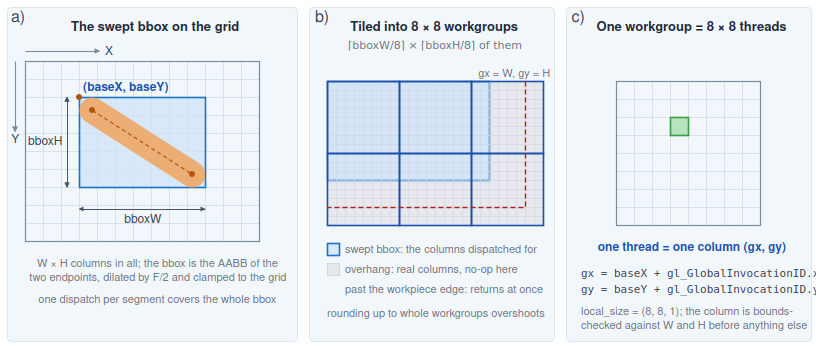
\includegraphics[width=5.83333in,height=2.47292in]{figures/image9.png}\end{center}



\textbf{Fig. 5} Mapping compute threads onto the workpiece column grid.
(a) The host restricts the dispatch to the swept bounding box, the AABB
of the segment endpoints dilated by F/2 and clamped to the grid, giving
the origin (baseX, baseY) and the size bboxW × bboxH. (b) The box is
tiled into ⌈bboxW/8⌉ × ⌈bboxH/8⌉ workgroups of 8×8 threads; rounding up
overshoots, so the last workgroups cover columns outside the box, and
those past the edge of the workpiece return immediately. (c) Each thread
handles one column, recovered from its global invocation ID

\hypertarget{the-subtract_swept-shader-step-by-step}{%
\subsubsection{4.4 The subtract\_swept shader, step by
step}\label{the-subtract_swept-shader-step-by-step}}

Each thread runs the following steps (Fig. 6). The shader is
deliberately branch-light and reads the tool from cached buffers, while
the large obj1\_flat buffer is read once and written once per column.

\begin{enumerate}
\def\labelenumi{\arabic{enumi}.}
\item
  Identify the column: recover gx = baseX+gl\_\allowbreak GlobalInvocationID.x and
  gy = baseY+gl\_\allowbreak GlobalInvocationID.y from the thread\textquotesingle s
  position in the dispatch (§4.3), and return immediately if gx ≥ W or
  gy ≥ H.
\end{enumerate}

\begin{enumerate}
\def\labelenumi{\arabic{enumi}.}
\setcounter{enumi}{1}
\item
  Read the stock column: its transition count count1 from obj1\_dataNum,
  and its transitions from obj1\_flat.
\end{enumerate}

\begin{enumerate}
\def\labelenumi{\arabic{enumi}.}
\setcounter{enumi}{1}
\item
  Bound the sub-step range {[}k0, k1{]}: the sub-positions of the tool
  centre for which the tool could cover this column (the sub-positions
  being tr = start + round(k*Δ/K), component-wise nearest integer, for k
  = 0\ldots K).
\item
  Accumulate the Z-envelope: loop k over {[}k0, k1{]}; for each, find
  the tool\textquotesingle s column under (gx, gy) and update zbMin =
  min(zbMin, bottom), ztMax = max(ztMax, top).
\item
  Tube-pruning early-out: if enableSkip and (the envelope accumulated no
  coverage over the whole sub-step range, hasMat == false, or the
  interval {[}zbMin, ztMax{]} lies entirely outside {[}0, z1)), return
  without writing (§3.6).
\item
  Subtract: perform a two-pointer merge of the stock column with the
  single interval {[}zbMin, ztMax{]}, emitting a transition whenever the
  result occupancy (stockInside AND NOT toolInside) changes.
\item
  Write back the result transitions in place, zero the unused slots
  (optional; §6.4), and store the new count.
\item
  Optional counter: when material-removal tracking is enabled, the
  shader measures the column\textquotesingle s solid extent before and
  after the merge and performs atomicAdd(removed{[}segment{]}, oldSolid
  - newSolid). This gives the volume removed by each segment, which the
  optimization loop of §1.1 uses to score candidate toolpaths.
\end{enumerate}

\begin{center}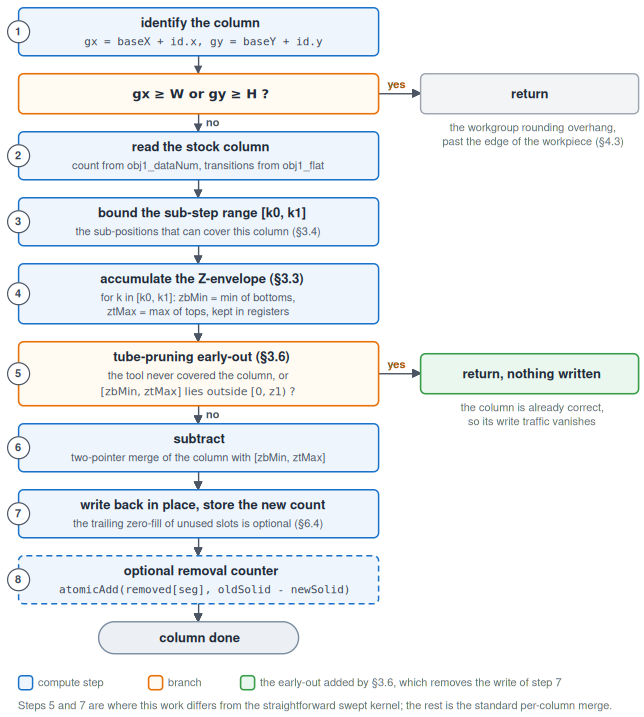
\includegraphics[width=5.83333in,height=6.49375in]{figures/image10.png}\end{center}



\textbf{Fig. 6} Per-thread control flow of subtract\_swept.comp, with
the step numbers of §4.4. One GPU thread handles one column, and every
column of the swept bounding box runs this independently. The two exits
leave without writing: the first on the workgroup rounding overhang past
the edge of the workpiece (§4.3), the second on the tube-pruning
early-out of step 5 (§3.6), which is what removes the write-back of step
7 for columns the tool never touches

Two design points matter for performance. The merge is in place: the
column is read once and written once, with no round-trip through an
intermediate swept solid, and the envelope is built from the tool
column\textquotesingle s lowest and highest transitions rather than from
a materialized volume. The write of step 7 covers the whole
MAX\_TRANSITIONS stride, which is what makes it the expensive part of
the thread and why removing it matters twice over: the early-out of step
5, the only change that §3.6 makes to the shader, skips it entirely for
columns the tool never touches, and dropping the trailing zero-fill
(§6.4) shortens it for the columns it does touch. The optional counter
of step 8 is gated by a uniform and off in every run reported here, so
neither the atomic nor the two extra column scans that feed it appear in
the timings.

\hypertarget{tool-geometry}{%
\subsubsection{4.5 Tool geometry}\label{tool-geometry}}

A ball-end mill is not a sphere but a cylinder with a hemispherical tip,
and its shank rises above the stock: in normal 3-axis milling it is out
of the workpiece at every instant, so the shank top, though a genuine
transition in the tool\textquotesingle s representation, always falls
outside the stock\textquotesingle s {[}0, z1) range and is dropped when
the removed interval is clamped to that range (§3.3, §4.4).

The method is exact for the tools of §3.3, whose columns are single
Z-intervals. It is worth being precise about where the approximation
would arise. At a single tool position, for a convex-in-Z tool, each
column has exactly two transitions, so representing it as {[}bottom,
top{]} loses nothing: a per-step stamper merging the
tool\textquotesingle s full transition list reads exactly those two
values and no others. The reduction is real only because {[}zbMin,
ztMax{]} is the union over all the sub-positions of a segment, and
convexity in Z is what guarantees that union is again a single interval.

For a tool that is not convex in Z the guarantee fails, and the envelope
treats any internal gap along Z as solid. The error is one-sided: an
over-removal equal to the volume of those gaps swept along the path. It
is a property of the tool rather than of the toolpath: a tool with no
internal gaps is exact; one with them is wrong by the same amount on
every segment that engages the material. A per-step stamper does not
share this artefact, since it never forms the union, though it differs
from the swept result for the separate reason given in §4.6. Undercut
geometries are outside the scope of a single-axis dexel field, since a
column stores only Z-transitions.

\hypertarget{correctness-byte-identity-exactness-and-the-gap-to-the-continuum}{%
\subsubsection{4.6 Correctness: byte-identity, exactness, and the gap to
the
continuum}\label{correctness-byte-identity-exactness-and-the-gap-to-the-continuum}}

Three claims hold, of decreasing strength, and it is worth separating
them.

(i) The swept optimizations are byte-identical to one another. The
external-buffer (S1), fused (S2) and tube-pruned (S3) kernels produce
byte-identical carved output, since pruning only skips writes to columns
it leaves unchanged. This is the load-bearing correctness claim: it
shows that the fusion and the pruning change nothing geometric. We
verify it by a direct diff of the saved .bin files (§5.3).

(ii) The envelope is exact with respect to stamping on the same sample
grid. Set difference distributes over unions and is order-independent,
so A\textbackslash(B₁∪\ldots∪Bₙ) =
(\ldots((A\textbackslash B₁)\textbackslash B₂)\ldots\textbackslash Bₙ),
and the swept volume is the union of the tool at the sub-positions
sampled along the segment. Those are taken at Chebyshev step K =
max(\textbar Δx\textbar,\textbar Δy\textbar,\textbar Δz\textbar), the L∞
length, giving tr = start+round(k*Δ/K) for k = 0\ldots K, consecutive
positions differing by at most one voxel per axis. Collapsing the tool
column to a single interval therefore loses nothing: at each
sub-position a convex-in-Z column already has exactly two transitions
(§4.5), and their union over the segment is again one interval. The
argument is verified directly: stamping the tool\textquotesingle s full
transition list at exactly those positions produces output
byte-identical to the envelope, on an axis-aligned and on a 45° segment.

(iii) Against the continuous sweep the envelope is exact on axis-aligned
moves and under-removes slightly on diagonals. The reference here is
analytic, not a finer stamper: for a linear segment the squared lateral
distance from a column to the tool axis is a quadratic in the
interpolation parameter, so the deepest coverage of every column has a
closed form, and the exactly swept solid can be computed without
sampling. Measured against it, on a 600-voxel segment, the kernel
removes 248,432 voxels against 248,432 exact on the axis-aligned move, a
gap of zero, and 349,574 against 349,855 at 45°, an under-removal of
0.080 \%. The axis-aligned result is structural rather than fortuitous:
there the integer sub-steps fall on every position the
continuum\textquotesingle s deepest coverage requires. On a diagonal the
true closest approach lies at a fractional centre between two integer
samples, so the column is cut a fraction of a voxel shallower. The gap
is a discretisation artefact and vanishes with the voxel: on the same
segment it is 0.450 \% at twice the voxel size, 0.080 \% at the native
one, 0.027 \% at half and 0.010 \% at a third. The trend is computed on
an emulation of the kernel that is byte-exact against the GPU at the
native resolution: the comparison cannot be repeated on hardware at
other resolutions, because the tool must be re-voxelised at each one,
and the resulting change in its discretised profile is two orders of
magnitude larger than the sampling term it would be measuring.

Two quantities must be kept out of this figure. The first is the
voxelised tool itself, which differs from the ideal hemisphere it
approximates by an amount that depends on the tool file and its radius,
about 1.4\% for the tool used here; that is a property of the tool
model, it cancels in any comparison between two carvers using the same
tool, and it is not an algorithm error, so the reference above holds the
depth profile fixed and compares only the sampling in t. The second is
the -\/-legacy stamper, which is a coarser reference on a different
lattice: it advances by Euclidean arc length and truncates towards zero,
where the swept path rounds to nearest on the Chebyshev grid. That is
why the two are not byte-identical at any step we tested, and why a
stray comparison between them mixes lattice geometry with the sampling
gap.

One implementation artefact in that path has also been corrected: its
drive loop advanced before stamping and so skipped each
segment\textquotesingle s first sample. The fix stamps the start once,
up front, and changes no timing figure. We therefore use S0 as a timing
and behavioural reference, not a geometric ground truth.

All volume comparisons use one invariant, the residual solid volume, the
sum over all columns and their solid intervals of (top - bottom), a
deterministic and render-independent quantity; the byte comparisons are
direct diffs of the saved files.

\hypertarget{numerical-experiments}{%
\subsection{5. Numerical experiments}\label{numerical-experiments}}

\hypertarget{hardware-software-and-the-ab-toggle}{%
\subsubsection{5.1 Hardware, software, and the A/B
toggle}\label{hardware-software-and-the-ab-toggle}}

Measurements are on an Intel Lunar Lake integrated GPU (Mesa iris
driver), OpenGL 4.6 compute, which the simulator reaches via an
EGL/Wayland context. Every level runs from the same binary and is
selected at runtime, which is essential for a fair A/B: -\/-legacy gives
S0, -\/-legacy-external-buffer gives S1, and the fused kernel gives S2
with SWEPT\_SKIP=0 or S3 with =1, the default. All runs are headless
(-\/-no-view), and timings are the interleaved mean-of-N described in
§5.4.

\hypertarget{benchmarks-and-the-g-code-generator}{%
\subsubsection{5.2 Benchmarks and the G-code
generator}\label{benchmarks-and-the-g-code-generator}}

The optimization targets segments whose length L exceeds the tool
footprint F, and its effect depends on the orientation of those
segments, so the benchmark programs are synthetic: each isolates one
point in that space rather than averaging over the mixture a production
part would contain. Two ball-end tool models are used, distinguished by
their footprint in voxels, one 256 wide and one 32 wide. With the wide
tool a segment of a few hundred voxels is comparable to the footprint,
so the dispatch bounding box already coincides with the swept band; with
the narrow one the same geometry gives L \textgreater\textgreater{} F.
All programs run on the same stock, a prismatic block of 1000×1000×500
voxels, which we refer to as the reference stock throughout. Everything
below is expressed in voxels, and deliberately so: the cost of a carve
is set by the number of columns touched and by the ratio L/F, not by the
physical size of the part, so a millimetre scale would add a constant
without changing any of the comparisons. The tools are likewise
described by their footprint in voxels.

\begin{itemize}
\item
  Axis-aligned perimeter (\texttt{square\_600}), with the 256-voxel tool
  (\texttt{mill\_10}): a closed square perimeter of side 600 voxels, cut
  along the axes. This is the control, chosen because its cutting
  segments are axis-aligned and short relative to the footprint, so
  per-column pruning has little off-band material to skip. The same
  perimeter cut with the 32-voxel tool (\texttt{mill\_3}) is
  \texttt{contour} in Table 3; the pair isolates the L/F ratio on one
  fixed geometry.
\item
  Diagonal cuts (\texttt{diag\_cut}) and air-heavy travel
  (\texttt{air\_moves}), with the 32-voxel tool: two micro-benchmarks
  that isolate the two effects. \texttt{diag\_cut} is a boustrophedon of
  long diagonal cuts, where the endpoint bounding box (≈ L²/2) dwarfs
  the swept band (≈ L*F) and per-column pruning skips the off-band
  columns. \texttt{air\_moves} is an air-heavy program (short diagonal
  cuts reached by long diagonal in-air rapids), where the whole dispatch
  of each rapid is skipped. The mixed 45° raster that combines cutting
  and air travel in one program is \texttt{raster45} in Table 3 (§6.1);
  its S2→S3 gain there is the same lever measured on the same diagonal
  geometry, not independent evidence.
\end{itemize}

The carved result of every program is rendered in Appendix B. The
diagonal programs are emitted by a small parametric generator that walks
lanes in a rotated basis (cutting direction \textbf{$\hat{u}$} = {[}1/√2,
1/√2{]}, step direction \textbf{$\hat{v}$} = {[}1/√2, -1/√2{]}), converting each
{[}u, v{]} to {[}x, y{]}; every generated file records its exact
regeneration command in its header. The programs, tool models and
benchmark scripts are available with the code (see the data availability
statement).

\hypertarget{validation}{%
\subsubsection{5.3 Validation}\label{validation}}

For every configuration we save the carved .bin. Across the three swept
levels - external-buffer S1, fused S2, pruned S3, the file is
byte-identical, which is what certifies that the fusion and the pruning
leave the geometry untouched; the comparison is a direct diff of the
files. The stamper S0 is a coarser reference, not a ground truth: it is
not byte-identical to the swept output at any step we tested (2, 1, 0.5,
0.25 voxels), because it samples a different lattice (§4.6). Against the
analytic continuum reference of that section the swept result is exact
on an axis-aligned segment and under-removes by 0.08 \% on a 45° one. As
a second, independent check, the residual solid volume of the carved
result is recomputed offline by a pure-Python reader with no dependency
on the GPU path, and agrees on both a perimeter program (281,165,072
voxels) and a star-shaped pocket (462,722,118). The latter is not one of
the benchmark programs of §5.2; it is a concave pocket kept as a
regression case.

\hypertarget{methodology}{%
\subsubsection{5.4 Methodology}\label{methodology}}

Each configuration is run eleven times; the first run is discarded as
compute-pipeline warm-up and the arithmetic mean of the remaining ten
net-carving times is reported (the GPU timings fluctuate run-to-run, so
the mean is more representative than a single minimum). Crucially, the
modes are interleaved per round (one run of each mode per round) rather
than measured in separate batches, so that GPU clock and thermal drift
cancel in the ratio: without this, measuring the modes in separate
batches made the never-taken branch of the axis-aligned control appear
about 30 \% slower. Timing uses the simulator\textquotesingle s internal
net-carving timer, a glFinish around the per-segment loop, excluding
read-back.

To turn these per-campaign means into publishable figures with error
bars, the entire suite was run as ten independent campaigns on an
otherwise idle machine (load average below one), and every number
reported in §6 is the mean over the ten campaigns, quoted with the
population standard deviation across them - so each figure is a mean of
ten × ten = one hundred carves, and the stated spread is run-to-run
reproducibility rather than within-run jitter. Across the ten campaigns
the coefficient of variation of every reported mean stays below about
six percent. Ratios are formed within each campaign and then averaged,
so they do not exactly equal the ratio of the rounded means shown in the
tables.

One measurement effect must be kept in view when reading the absolute
times. The net time of a given swept level depends on the mix of modes
interleaved with it, not only on the kernel: the same S2 kernel on
square\_600 reads about 17.6 ms inside the four-level sweep of Table 2,
where each round is dominated by the roughly 520 ms legacy stamp that
lets the integrated GPU recover between swept runs, but about 32 ms when
only S2 and S3 are interleaved back-to-back and the GPU stays in a
hotter clock state. The cross-campaign spread of each of those figures
is under two percent, so this is a clock/thermal (DVFS) effect of the
integrated GPU, not load noise. Ratios cancel it; we therefore state
every speed claim as a ratio and compare absolute times only within a
single table. The pruning ratio on the axis-aligned control is
additionally reported from a standalone high-N run (thirty measurements
per campaign) that isolates it from that recovery.

\hypertarget{results}{%
\subsection{6. Results}\label{results}}

The four levels of §1.3 are measured in two groups. Table 1 isolates the
pruning lever, S2→S3, on the two generated diagonal stress programs; the
axis-aligned control spans that L/F regime as the four-level ablation of
Table 2. Table 3 then measures all four levels on the same six machining
workloads, which separates what the literature already delivers, the
per-move swept formulation (S0→S1), from this work\textquotesingle s
fusion of the subtraction (S1→S2) and its pruning (S2→S3); that matrix
is the primary comparison. Table 2 is the four-level end-to-end ablation
on the axis-aligned control, from the naive stamper (S0) to this
work\textquotesingle s pruned kernel (S3). The memory side is
consolidated in §6.3 and the sparse tiled working set in §6.2.

\textbf{Table 1} Tube pruning on the two diagonal stress benchmarks: net
carving time (ms), Intel Lunar Lake / iris, mean of ten interleaved
campaigns ± population sd (§5.4), S2 and S3 byte-identical. "S2 swept"
is the fused baseline of §3.3; "S3 +pruning" is this work. diag\_cut
isolates the per-column pruning of off-band columns; air\_moves isolates
the whole-dispatch air-skip of in-air rapids. The axis-aligned control,
whose dispatch bounding box already nearly matches the swept band with
the 256-voxel tool, is the four-level ablation of Table 2; with the
32-voxel tool the same per-column skip test costs at most ≈8 \% on dense
rasters (Table 3).

\begin{longtable}[]{@{}
  >{\raggedright\arraybackslash}p{(\columnwidth - 6\tabcolsep) * \real{0.4384}}
  >{\raggedright\arraybackslash}p{(\columnwidth - 6\tabcolsep) * \real{0.1912}}
  >{\raggedright\arraybackslash}p{(\columnwidth - 6\tabcolsep) * \real{0.2057}}
  >{\raggedright\arraybackslash}p{(\columnwidth - 6\tabcolsep) * \real{0.1647}}@{}}
\toprule\noalign{}
\begin{minipage}[b]{\linewidth}\raggedright
Benchmark (tool)
\end{minipage} & \begin{minipage}[b]{\linewidth}\raggedright
S2 swept (baseline)
\end{minipage} & \begin{minipage}[b]{\linewidth}\raggedright
S3 +pruning (ours)
\end{minipage} & \begin{minipage}[b]{\linewidth}\raggedright
S2→S3
\end{minipage} \\
\midrule\noalign{}
\endhead
\bottomrule\noalign{}
\endlastfoot
diag\_cut (mill\_3, diagonal cuts) & 32.8 ± 1.5 & 10.1 ± 0.3 & 3.23× \\
air\_moves (mill\_3, air-heavy) & 39.0 ± 1.9 & 5.3 ± 0.4 & 7.45× \\
\end{longtable}

\begin{center}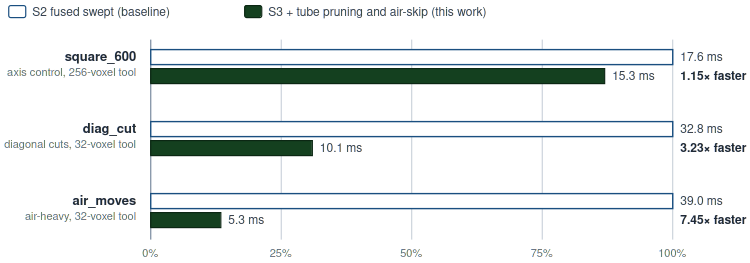
\includegraphics[width=6.26806in,height=2.19792in]{figures/image12.png}\end{center}



\textbf{Fig. 7} Tube pruning on the stress benchmarks, normalized to the
fused S2 baseline; shorter is faster. Net carving time, Intel Lunar Lake
/ iris, mean of ten campaigns (§5.4), byte-identical output. S3 wins
large on diagonal cutting (diag\_cut) and in-air work (air\_moves); the
axis-aligned control (square\_600) barely moves - 1.15× here (Table 2),
because with the 256-voxel tool the dispatch bounding box already nearly
matches the swept band. Mean of ten campaigns ± sd (§5.4)

Table 2 gives the four-level end-to-end ablation on the axis-aligned
control, from the naive stamper (S0) through the two established swept
baselines (S1, S2) to this work\textquotesingle s pruned kernel (S3), in
net carving and in total wall time including read-back.

\textbf{Table 2} Four-level ablation on the control (square\_600,
mill\_10): net carving and total time including read-back, mean of ten
interleaved campaigns ± population sd (§5.4). S1--S3 are byte-identical;
S0 is a coarse, differently-sampled reference, not a geometric ground
truth (§4.6). Overall S0→S3 is 34.2 ± 0.7× in net carving (17.1 ± 0.3×
including read-back), and the fusion step S1→S2 is 1.54 ± 0.03×. Pruning
on this axis-aligned control (S2→S3) is a modest 1.15 ± 0.02× as
measured inside the sweep, rising to 1.25 ± 0.01× in a standalone high-N
run (N = 30 per campaign) that removes the clock recovery the long S0
stage affords between swept runs (§5.4).

\begin{longtable}[]{@{}
  >{\raggedright\arraybackslash}p{(\columnwidth - 4\tabcolsep) * \real{0.3999}}
  >{\raggedright\arraybackslash}p{(\columnwidth - 4\tabcolsep) * \real{0.2999}}
  >{\raggedright\arraybackslash}p{(\columnwidth - 4\tabcolsep) * \real{0.3002}}@{}}
\toprule\noalign{}
\begin{minipage}[b]{\linewidth}\raggedright
Level
\end{minipage} & \begin{minipage}[b]{\linewidth}\raggedright
Net carving (ms)
\end{minipage} & \begin{minipage}[b]{\linewidth}\raggedright
Total incl. read-back (ms)
\end{minipage} \\
\midrule\noalign{}
\endhead
\bottomrule\noalign{}
\endlastfoot
S0 - per-step stamping {[}1{]} & 522.3 ± 2.6 & 549.5 ± 2.0 \\
S1 - swept, external buffer {[}2--4{]} & 27.1 ± 0.6 & 46.4 ± 1.1 \\
S2 - swept, fused in place (this work) & 17.6 ± 0.4 & 34.4 ± 0.7 \\
S3 - + tube pruning + air-skip (this work) & 15.3 ± 0.3 & 32.2 ± 0.6 \\
\end{longtable}

Overall S0→S3 is 34.2× in net carving (17.1× with read-back). The
pruning of §3.6 is applied on top of the S2 swept baseline. Because
Table 2 uses \texttt{square\_600} with the larger \texttt{mill\_10}
tool, its absolute milliseconds differ from the \texttt{mill\_3}
net-carving figures in Tables 1 and 3; the comparison of interest is
always within a table, on one binary and hardware.

\hypertarget{cross-workload-matrix-established-methods-vs.-this-work}{%
\subsubsection{6.1 Cross-workload matrix: established methods vs.~this
work}\label{cross-workload-matrix-established-methods-vs.-this-work}}

Table 1 isolates the pruning lever on two diagonal stress programs; to
separate what a \emph{known} method already buys from this work's
contributions across realistic work, we ran a suite of machining
workloads that stress different axes at four refinement levels, all on
the same binary, representation and GPU - apples-to-apples. We
deliberately do not quote other authors' absolute timings (meaningless
across hardware, representation, tool and resolution); each level is
\emph{our} fair, optimized implementation of the corresponding algorithm
class, anchored to the literature it represents:

\begin{itemize}
\tightlist
\item
  S0, per-step stamping: the classic z-map/dexel display method (Van
  Hook 1986 {[}1{]}); the tool is stamped at fixed jog steps along each
  segment (\texttt{-\/-legacy}, default step 2 voxels - the setting a
  display-oriented stamper would realistically use). S0 is a timing and
  behavioural reference, not a geometric ground truth (§4.6).
\item
  S1, swept, external buffer: the straightforward per-move swept
  implementation (the multi-/tri-dexel class; Müller \& Surmann 2003
  {[}2{]}; Tukora \& Szalay 2012 {[}3{]}; Inui et al.~2019 {[}4{]}) -
  the swept volume is materialized in a separate full-size buffer and
  then subtracted (\texttt{-\/-legacy-external-buffer}).
\item
  S2, swept, fused in-place: this work's fusion - the swept-tool column
  is computed on the fly as a Z-envelope and subtracted in place in the
  resident buffer, with no intermediate swept-volume buffer (§3.3;
  \texttt{SWEPT\_SKIP=0}).
\item
  S3, + tube pruning + in-air skip: this work\textquotesingle s traffic
  pruning on top of S2 (§3.6).
\end{itemize}

The design decision the paper claims - fuse the subtraction rather than
materialize the swept volume - is thus isolated as a single measured
step, S1→S2. The three swept levels (S1--S3) are byte-identical to one
another; S0 is a timing and behavioural reference, not a geometric
ground truth (§4.6).

\textbf{Table 3} Net carving time (ms) per machining workload and
refinement level (32-voxel tool; mean of ten interleaved campaigns ±
population sd, cross-campaign CV ≤ 6\% (§5.4), Intel iris; swept levels
byte-identical, S0 a coarse reference not a ground truth). S1→S2 is the
fusion / no-external-buffer gain (this work); S2→S3 is pruning (this
work); S0→S3 is overall.

\begin{longtable}[]{@{}
  >{\raggedright\arraybackslash}p{(\columnwidth - 14\tabcolsep) * \real{0.1942}}
  >{\raggedright\arraybackslash}p{(\columnwidth - 14\tabcolsep) * \real{0.1049}}
  >{\raggedright\arraybackslash}p{(\columnwidth - 14\tabcolsep) * \real{0.1535}}
  >{\raggedright\arraybackslash}p{(\columnwidth - 14\tabcolsep) * \real{0.0806}}
  >{\raggedright\arraybackslash}p{(\columnwidth - 14\tabcolsep) * \real{0.0971}}
  >{\raggedright\arraybackslash}p{(\columnwidth - 14\tabcolsep) * \real{0.1050}}
  >{\raggedright\arraybackslash}p{(\columnwidth - 14\tabcolsep) * \real{0.0971}}
  >{\raggedright\arraybackslash}p{(\columnwidth - 14\tabcolsep) * \real{0.1676}}@{}}
\toprule\noalign{}
\begin{minipage}[b]{\linewidth}\raggedright
Workload (what it stresses)
\end{minipage} & \begin{minipage}[b]{\linewidth}\raggedright
S0
\end{minipage} & \begin{minipage}[b]{\linewidth}\raggedright
S1
\end{minipage} & \begin{minipage}[b]{\linewidth}\raggedright
S2
\end{minipage} & \begin{minipage}[b]{\linewidth}\raggedright
S3
\end{minipage} & \begin{minipage}[b]{\linewidth}\raggedright
S1→S2
\end{minipage} & \begin{minipage}[b]{\linewidth}\raggedright
S2→S3
\end{minipage} & \begin{minipage}[b]{\linewidth}\raggedright
S0→S3
\end{minipage} \\
\midrule\noalign{}
\endhead
\bottomrule\noalign{}
\endlastfoot
what the level is & stamping & swept, ext. buffer & swept, fused & +
prune + air-skip & (fusion) & (prune) & \\
attribution & Van Hook {[}1{]} & straightforward swept {[}2--4{]} & this
work & this work & & & \\
contour - axis-aligned perimeter & 51.47 & 10.00 & 4.01 & 4.08 & 2.49× &
0.99× & 12.6× \\
pocket\_axis - axis-aligned raster & 151.22 & 17.81 & 8.76 & 9.25 &
2.03× & 0.95× & 16.4× \\
raster45 - 45° diagonal raster & 264.75 & 43.88 & 35.59 & 14.79 & 1.23×
& 2.41× & 17.9× \\
rapids - scattered cuts, long air moves & 81.00 & 17.41 & 12.76 & 6.63 &
1.37× & 1.93× & 12.2× \\
localized - small corner feature & 39.00 & 13.46 & 5.77 & 4.92 & 2.34× &
1.18× & 7.9× \\
finishing - fine-stepover axis-aligned raster & 111.57 & 15.36 & 7.60 &
8.18 & 2.02× & 0.93× & 13.7× \\
\end{longtable}

Two of the levels are established, two are ours. S0→S1 (≈2.9-8.5×) is
the per-move swept formulation over per-step stamping - what the known
methods already deliver. S1→S2 (≈1.2--2.5×, geomean ≈1.85×) is this
work's fusion: computing the swept envelope on the fly and subtracting
it in place, rather than writing it to a separate buffer and subtracting
in a second pass, is a consistent speed win \emph{and} removes a
full-size resident buffer (§6.3) - the gain is largest where the carve
is otherwise cheap (the fixed cost of the extra pass and buffer
round-trip dominates) and smallest on the big diagonal raster. S2→S3 is
this work's tube pruning, workload-dependent by construction: it removes
the over-dispatch of \emph{non-axis-aligned} segments (45° raster 2.41×)
and \emph{in-air} rapids (1.93×), and on axis-aligned programs it costs
at most ≈8 \% (contour 0.99×, pocket\_axis 0.95×, finishing 0.93×) - the
price of the per-column branch on dense rasters where every column is
active and the AABB already equals the swept band. Fusion (S1→S2) and
pruning (S2→S3) are complementary - the first always pays, the second
pays where the dispatch over-covers. Reproducible via
\texttt{tools/bench\_matrix.sh}.

\begin{center}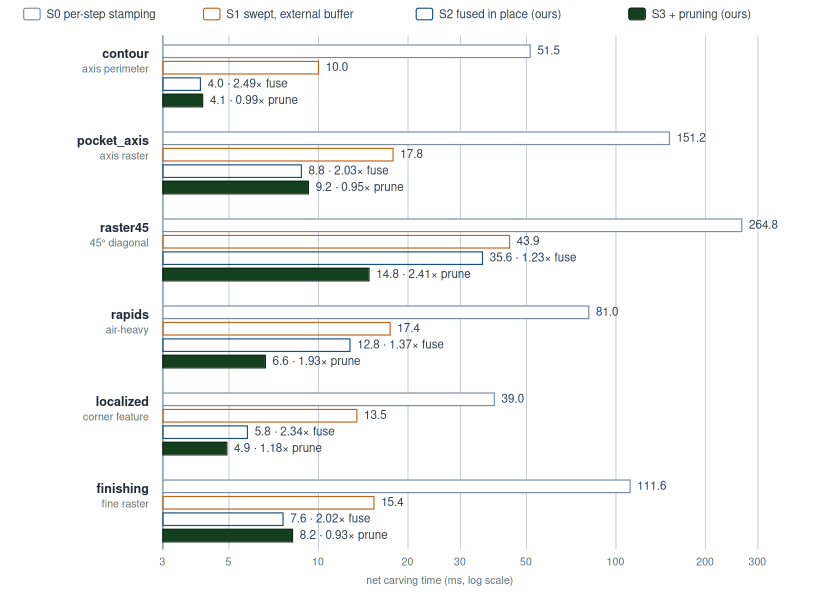
\includegraphics[width=6.26806in,height=4.53333in]{figures/image14.png}\end{center}

\textbf{Fig.
8} Net carving time per machining workload and refinement level (log
scale). S0→S1 is the established per-move swept method; S1→S2 is this
work's fusion - the swept volume computed on the fly and subtracted in
place instead of via a separate buffer (≈1.2-2.5×, and it halves
resident memory); S2→S3 is this work's tube-pruning + in-air skip, which
pays where the dispatch over-covers (45° raster 2.41×, air-heavy 1.93×)

\hypertarget{working-set-a-sparse-tiled-study}{%
\subsubsection{6.2 Working-set: a sparse tiled
study}\label{working-set-a-sparse-tiled-study}}

The 128 MB flat buffer is \textasciitilde16× padding
(\texttt{MAX\_TRANSITIONS\ =\ 32} vs.~2 to 4 real transitions per
column). A full alternative backend (\texttt{CARVE\_BACKEND=sparse})
stores the stock in \texttt{32×32}-column tiles, keeping untouched tiles
UNIFORM (O(1)) and materializing a tile only when a segment's bounding
box first touches it - byte-identical to the flat backend,
runtime-selectable. It isolates two effects. (i) Per-carve bandwidth is
bounded by the \emph{swept bounding box}, not the buffer size (both
backends touch only the bbox columns), so tiling does not reduce the
carve's traffic \emph{volume}; it only improves access \emph{locality}
(the strided-access problem) → \textasciitilde1.1× (square\_600 1.09×,
raster45 1.11×, pocket\_axis 1.15×). (ii) Footprint is a conditional win
tied to locality - a localized program materializes 49-56 / 1024 tiles
(8 MB vs.~122 MB, \textasciitilde15×), whereas whole-stock machining
touches most tiles (raster45 736 / 1024, no saving). So sparse tiling is
a memory/scale lever (finer resolutions, larger stocks, smaller
read-back for localized work), not a carve-speed lever; host-side
materialization even makes whole-stock programs slower.

\hypertarget{memory-and-data-movement-across-the-four-levels}{%
\subsubsection{6.3 Memory and data movement across the four
levels}\label{memory-and-data-movement-across-the-four-levels}}

Speed is only half the story: each step also shrinks what the GPU must
hold and move. Table 4 consolidates the footprint and data-movement
figures introduced piecemeal above (§3.3, §3.5, §6.2) for the reference
stock.

\textbf{Table 4} Resident footprint and data movement, per level
(reference stock)

\begin{longtable}[]{@{}
  >{\raggedright\arraybackslash}p{(\columnwidth - 8\tabcolsep) * \real{0.2247}}
  >{\raggedright\arraybackslash}p{(\columnwidth - 8\tabcolsep) * \real{0.1896}}
  >{\raggedright\arraybackslash}p{(\columnwidth - 8\tabcolsep) * \real{0.2226}}
  >{\raggedright\arraybackslash}p{(\columnwidth - 8\tabcolsep) * \real{0.1805}}
  >{\raggedright\arraybackslash}p{(\columnwidth - 8\tabcolsep) * \real{0.1827}}@{}}
\toprule\noalign{}
\begin{minipage}[b]{\linewidth}\raggedright
\end{minipage} & \begin{minipage}[b]{\linewidth}\raggedright
Naive stamping
\end{minipage} & \begin{minipage}[b]{\linewidth}\raggedright
Swept, external buffer (S1)
\end{minipage} & \begin{minipage}[b]{\linewidth}\raggedright
Fused in place (S2)
\end{minipage} & \begin{minipage}[b]{\linewidth}\raggedright
+ pruning (S3)
\end{minipage} \\
\midrule\noalign{}
\endhead
\bottomrule\noalign{}
\endlastfoot
\textbf{Material-to-remove} & tool stamped every jog step & materialized
- swept volume written to a buffer & none - O(1) Z-envelope per column,
on the fly & same as S2 \\
\textbf{Resident working set} & 128 MB flat & 256 MB - 128 MB stock + a
128 MB swept twin & 128 MB (no twin) & 8 MB sparse for localized work
(\textasciitilde15×), else 128 MB \\
\textbf{Result assembly} & separate output + per-step 12 MB stock copy &
second pass reads the twin, subtracts & in place in the one working
buffer & same as S2 \\
\textbf{Read-back transfer} & 128 MB unpacked & 8 MB GPU-compacted & 8
MB GPU-compacted (\textasciitilde16×) & same as S2 \\
\textbf{Per-carve write traffic} & whole grid, full footprint &
swept-AABB columns, twice (write twin + subtract) & swept-AABB columns,
once & swept tube only - off-band / off-Z columns skipped \\
\end{longtable}

The fusion (S1→S2) is a memory decision as much as a speed one: the
external-buffer baseline needs a full-size 128 MB twin of the working
buffer to hold the materialized swept volume (2× resident), and
round-trips the envelope through it, whereas the fused kernel keeps only
an O(1) per-column envelope in registers - so it halves resident memory
while also running 1.2--2.5× faster across the matrix, geomean ≈1.85×
(§6.1), and 1.54× on the control (Table 2). The memory wins up to S2 are
unconditional (in-place single buffer, no per-step 12 MB stock copy, 8
MB compacted read-back); S3 adds a conditional footprint win tied to
spatial locality (§6.2) and a write-traffic reduction tied to
non-axis-aligned and in-air motion (§6.1). No step trades memory for
speed: the two move together, because the simulator is bandwidth-bound
(§7).

\hypertarget{dead-write-back-on-active-columns}{%
\subsubsection{6.4 Dead write-back on active
columns}\label{dead-write-back-on-active-columns}}

Every processed column writes its full \texttt{MAX\_TRANSITIONS}-slot
stride: \texttt{writeCount} real transitions, then zeros to the end
(§4.4). Occupancy reads only the first \texttt{obj1\_dataNum{[}col{]}}
slots, so those zeros are dead - a typical active column has 2--4
transitions, i.e.~\textasciitilde8 useful bytes of the 128 written.
Dropping the zero-fill (\texttt{SWEPT\_ZEROFILL=0}) is byte-identical
(verified by a \texttt{.bin} diff over the whole suite) and removes that
dead traffic on \emph{active} columns, the complement of tube pruning,
which removes traffic on \emph{inactive} ones.

On the fused kernel (pruning off) it removes real write traffic. Table 5
gives one interleaved session with three configurations side by side, so
every comparison below can be checked against it directly.

\textbf{Table 5} The zero-fill lever and the best available
configuration, from one interleaved loop within the campaign (32-voxel
tool, net carving ms, mean of ten campaigns ± sd, §5.4). Absolute times
differ from Tables 2--3 because this loop interleaves only cheap swept
configs, so the GPU stays in a hotter clock state (§5.4); the
comparisons of interest are within this table. The two S2 columns are
byte-identical (verified by a \texttt{.bin} diff). The pruned kernel
without zero-fill was measured in the same campaign and is discussed in
the text.

\begin{longtable}[]{@{}
  >{\raggedright\arraybackslash}p{(\columnwidth - 6\tabcolsep) * \real{0.2499}}
  >{\raggedright\arraybackslash}p{(\columnwidth - 6\tabcolsep) * \real{0.2500}}
  >{\raggedright\arraybackslash}p{(\columnwidth - 6\tabcolsep) * \real{0.2500}}
  >{\raggedright\arraybackslash}p{(\columnwidth - 6\tabcolsep) * \real{0.2500}}@{}}
\toprule\noalign{}
\begin{minipage}[b]{\linewidth}\raggedright
Workload
\end{minipage} & \begin{minipage}[b]{\linewidth}\raggedright
S2 (zero-fill)
\end{minipage} & \begin{minipage}[b]{\linewidth}\raggedright
S2 (no fill)
\end{minipage} & \begin{minipage}[b]{\linewidth}\raggedright
S3 (default)
\end{minipage} \\
\midrule\noalign{}
\endhead
\bottomrule\noalign{}
\endlastfoot
\texttt{contour} & 7.32 ± 0.18 & 6.76 ± 0.22 & 6.57 ± 0.21 \\
\texttt{pocket\_axis} & 18.30 ± 0.50 & 15.68 ± 0.53 & 17.63 ± 0.35 \\
\texttt{finishing} & 15.38 ± 0.42 & 13.04 ± 0.25 & 14.94 ± 0.37 \\
\texttt{raster45} & 43.86 ± 1.05 & 34.05 ± 0.87 & 18.70 ± 0.54 \\
\texttt{rapids} & 27.09 ± 0.79 & 24.16 ± 0.73 & 15.72 ± 0.51 \\
\texttt{localized} & 6.99 ± 0.21 & 6.46 ± 0.14 & 5.40 ± 0.25 \\
\end{longtable}

Dropping the zero-fill (columns one to two) is faster on every workload,
from 7.6 \% on the small localized program to 22 \% on the 45° raster;
the reduction is largest and most stable on the dense rasters
(\texttt{finishing} and \texttt{raster45}, 15--22\%), where the active
columns, and so the dead-write traffic, are most numerous. It is
byte-identical, and it acts on \emph{active} columns - the complement of
tube pruning's \emph{inactive}-column saving (§7). It is the
active-column lever the paper otherwise lacked, and it reaches the
axis-aligned case (\texttt{finishing}) where pruning is
neutral-to-negative (§6.1).

Columns two and three weigh the no-fill fused kernel against the shipped
pruned default. On axis-aligned work the two are close:
\texttt{finishing} is 15\% faster without pruning, while
\texttt{contour} and \texttt{pocket\_axis} fall within about 12\% either
way (contour favours the pruned default, pocket\_axis the no-fill
kernel). On non-axis-aligned and air-heavy work the default is far ahead
(1.8× on the 45° raster, 1.5× on the rapids). So the pruned default is
the right all-rounder, the no-fill fused kernel is competitive only on
dense axial work, and both are runtime-selectable.

Removing the zero-fill on the pruned kernel itself splits by workload,
exactly as the complementarity of §7 predicts. Where pruning has already
removed the off-band columns, on the diagonal and air-heavy programs,
little dead-write traffic remains and dropping the zero-fill is now
slightly counterproductive: raster45 and rapids both slow by about 3.5
\%, a small but reproducible regression consistent with the
partial-stride read-modify-write of §7. Where pruning finds nothing to
skip, on the dense axis-aligned rasters, the active columns and their
dead writes persist and removing the zero-fill still pays about 15 \%
(pocket\_axis and finishing). We keep the zero-fill on by default and
expose its removal as a toggle.

\hypertarget{discussion}{%
\subsection{7. Discussion}\label{discussion}}

The bottleneck is memory-write bandwidth. A design A/B and a series of
experiments, read together, localize it:

\begin{itemize}
\tightlist
\item
  Fusion vs.~an external buffer (positive, §6.1). Materializing the
  swept volume in a separate full-size buffer and subtracting it in a
  second pass round-trips the envelope through memory (write the twin,
  read it back) and doubles the resident set. Fusing the two - envelope
  on the fly, subtracted in place - removes that traffic and the twin,
  for a geomean ≈1.85× and half the memory. Removing memory traffic
  pays; the swept-envelope compute is identical in both, and it is not
  where the time goes.
\item
  Range-query envelopes (negative). Precomputing per-tool directional
  Z-envelopes as range-minimum/maximum sparse tables makes the
  per-column envelope an \texttt{O(1)} query instead of an
  \texttt{O(sub-steps)} loop. Implemented exactly, it gave a modest gain
  that did not justify the added structure, because it optimized
  compute, which is not the bottleneck, and was reverted.
\item
  Tube pruning (positive, §3.6). Skipping the write-back of off-band and
  out-of-Z-range columns attacks memory-write traffic and gives
  3.2--7.4× in its regime (stress benchmarks, Table 1). This is the
  complement of the previous result: the lever that pays removes memory
  traffic, not compute.
\item
  Dead-write elimination (positive on the fused kernel, §6.4). The
  trailing zero-fill of unused column slots is dead write traffic
  (\textasciitilde30 of 32 slots on a typical column). Dropping it is
  byte-identical and gives 8--22\% on the fused kernel - the
  active-column counterpart to tube pruning's inactive-column saving,
  and the one lever that reaches the axis-aligned case where pruning
  does nothing. It confirms the write-traffic diagnosis from the
  opposite side. The two do not add: they reduce traffic to the same
  buffer on complementary column sets, so once pruning has thinned the
  active set the remaining dead-write traffic is small and its removal
  drops into the noise (§6.4).
\item
  Oriented tiled dispatch (negative). Tempted to also avoid launching
  the off-band threads (each still does a counter read plus the
  early-out), we tiled the dispatch along the motion so it follows the
  band. Each tile reuses the full-segment envelope uniforms (so every
  column is computed identically); adjacent tiles overlap idempotently,
  separated by a barrier - keeping it byte-identical. The result was
  measurably slower than tube pruning alone: the per-tile barriers
  serialize the tiles and the joins double-process columns, and that
  synchronization cost exceeds the thread-launch saving, because tube
  pruning already made the off-band threads cheap (a read, no write).
  Reverted. Neither branch survives in the current build, so neither is
  measured on the benchmark set of §5.2 and neither appears in the
  tables; we report the direction of both results, which is what the
  diagnosis rests on, rather than figures from a configuration a reader
  could not reproduce.
\item
  Sparse tiled working-set (footprint, not speed; §6.2). A tiled backend
  that keeps untouched tiles UNIFORM shrinks the working set to the
  touched fraction, but the per-carve traffic is bounded by the swept
  bounding box in either layout, so it only improves access locality
  (\textasciitilde1.1×) and reduces footprint conditionally on locality
  (\textasciitilde15× localized, nothing whole-stock). Working-set size
  is a memory/scale lever, not a bandwidth one.
\end{itemize}

The pattern is consistent - a map of the bottleneck. Attacking compute
(RMQ), launched-thread count (tiled dispatch) or working-set size
(sparse tiling) yields diminishing, negative or footprint-only returns;
the levers that pay all remove memory-write traffic on the
over-dispatched bounding box - fusing away the swept-volume round-trip
(S1→S2, always), tube pruning the off-band/off-Z write-back on inactive
columns (S2→S3, where the dispatch over-covers), and dropping the dead
zero-fill on active columns (§6.4, the fused kernel). The granularity
that matters is the cache line: a column's 128-byte stride is two
64-byte lines, and a full-stride store writes both with no read, so the
payoff is in not touching a line - pruning skips both, the dead-write
removal skips the second. That is also why pruning and dead-write
removal overlap rather than add (same buffer, complementary columns),
and why a partial store that still touches the first line by
read-modify-write can fail to pay. The simulator is
bbox-bandwidth-bound, at cache-line granularity: the productive
optimization removes bbox lines touched. A dispatch-enqueue cost that
stays \textasciitilde0.4 ms whether a program has 9 or 202 segments
corroborates that per-segment host overhead is not the limit.

Portability and the roofline argument. All measurements here are on one
integrated GPU, which invites the question of whether the findings are
hardware-specific. They are not, and the reason is structural rather
than empirical. The per-column merge moves on the order of 128-256 bytes
per active column - it rewrites all \texttt{MAX\_TRANSITIONS\ =\ 32}
slots and reads a comparable number - while performing only a few
integer comparisons per 4-byte transition: an arithmetic intensity well
below 1 op/byte, one to three orders of magnitude under the ridge point
of any modern GPU roofline. A kernel this far into the memory-bound
regime is memory-bound on every GPU; and because discrete NVIDIA parts
carry a higher compute-to-bandwidth ratio than an integrated Intel GPU,
the diagnosis becomes more true there, not less. The load-bearing claims
are therefore architecture-invariant: the representation, the exactness
argument, the ``carving is a memory-movement problem'' thesis, and the
geometric workload dependence of tube pruning (a function of the
AABB-to-swept-band ratio, not the silicon) all transfer unchanged. The
pipeline also uses only portable compute primitives (SSBOs,
\texttt{std430}, dispatch, a storage barrier) - no subgroup intrinsics,
tensor or ray-tracing cores - so a Vulkan or CUDA port is a direct
transliteration of the same kernel.

A faster or discrete GPU changes magnitudes, not directions. Absolute
carve times fall with bandwidth while the kernel stays bandwidth-bound;
the fusion and pruning ratios shift because their fixed components (an
extra pass and a barrier for fusion; a per-column branch for pruning)
scale differently from the traffic they save - the fusion win is already
largest where the carve is cheapest, and that fixed-cost fraction only
grows as traffic gets faster. One optimization would become more
valuable off the iGPU: the GPU-side read-back compaction (128 MB → 8
MB), because on a discrete card the read-back crosses PCIe
(\textasciitilde16-32 GB/s), where the full unpacked buffer alone would
cost several milliseconds.

Three caveats are genuinely API-, occupancy- or driver-specific and
would warrant re-measurement. First, the oriented tiled dispatch
negative result is partly a statement about OpenGL\textquotesingle s
coarse glMemoryBarrier and dispatch model: CUDA and Vulkan expose finer
synchronization (timeline semaphores, cooperative groups, persistent
kernels, dynamic parallelism) that could avoid the barrier serialization
that sank it, so that reverted idea may be worth revisiting on those
APIs. Second, the per-thread localOut{[}64{]} scratch (256 B) and the
branchy sub-step loop interact with the register file and 32-wide warps:
register spilling or warp divergence could move the fine ratios, and the
large L2 caches of recent discrete GPUs (tens of MB) might hold more of
the active bounding box, plausibly increasing the sparse-tiling locality
benefit. Third, the sub-positions are computed in single precision and
rounded to nearest, and GLSL leaves the tie-break at exact half-integers
unspecified; a sample landing on or within an ulp of such a boundary can
resolve to either neighbour on a different driver. This never moves a
sample by more than one voxel and does not affect the byte-identity of
S1, S2 and S3 on one machine, which is what §5.3 verifies, but
byte-identity across drivers is not guaranteed. None of the three
changes which lever breaks the ceiling; together they set the agenda for
a cross-hardware study.

When tube pruning helps. The gain requires segment length
\texttt{L\ ≫\ F}. Axis-aligned programs, or diagonal programs machined
with a tool nearly as wide as the segments are long, see little - their
AABB already equals the tube. Real 3-axis programs, however, contain
substantial air travel (rapids between features, retract/reposition
links) and non-axis-aligned finishing toolpaths, all of which this
optimization accelerates; the in-air pruning in particular applies to
every rapid.

Limitations. The pipeline runs in voxel units. That is deliberate for
the results reported here (§5.2), but it does mean that a real G-code
program in millimetres is not yet consumed directly: the tool datum is
the centre of the tool\textquotesingle s bounding box, so the Z origin
shifts with the modelled shank length and neither the tip radius nor the
tool length is compensated. A calibrated millimetre mapping with an
explicit tool datum is future work. The envelope over-removes for
non-convex-in-Z tools, and the flat-buffer stride MAX\_TRANSITIONS = 32
is not overflow-guarded, though detection would be near-free to add
(§4.2). The tool is axis-fixed (3-axis only). Arcs are handled only as
polylines, so a segment count that grows with the chord tolerance is the
price of curved paths; a native circular-swept envelope would be a
natural extension. Against the continuously-swept cut the single-pass
envelope is exact on axis-aligned moves and under-removes by 0.08 \% on
a 45° one, a gap that shrinks with the voxel size (§4.6). The path used
when scoring a candidate toolpath is not itself optimized: the
per-segment removal counter is an unreduced global atomic per active
column on a single counter, plus two extra column scans, where a
per-workgroup shared-memory reduction would be the obvious fix; it is
disabled in all measurements reported here. That path is also where the
largest remaining lever lies: a GPU-side objective, comparing
carved-vs-target on the GPU, would remove the per-iteration read-back
entirely.

\hypertarget{conclusions}{%
\subsection{8. Conclusions}\label{conclusions}}

We presented a GPU material-removal simulator for 3-axis milling built
on a single-axis dexel field, in which Boolean difference is a
per-column merge that maps one workpiece column to one GPU thread. On
top of a fused, materialization-free swept-segment subtraction, we
introduced tube pruning - skipping the write-back for columns the swept
tool never touches - which is byte-identical and yields 3.2--7.4×
(stress benchmarks, Table 1) on the diagonal and air-heavy work that
dominates real toolpaths, with an axis-aligned effect that depends on
the program and tool (a gain when whole rapids are air-skipped or a
large-tool AABB overhangs the band, a modest cost on dense rasters where
every column is active). The optimization, two documented negative
results bracketing it, and a third positive one that removes the dead
per-column write-back on active columns, together show that in this
setting the decisive resource is memory-write bandwidth: the successful
levers remove bytes written, not arithmetic or launched threads. The
simulator is fast enough, and accurate against the continuously-swept
cut - exactly so on axis-aligned moves and to within 0.08 \% on
diagonals (§4.6) - to serve as a drop-in accelerator wherever repeated
carving simulation is the bottleneck, from interactive toolpath
verification to cutting-force models and search- or learning-based
toolpath optimization.

\hypertarget{appendix-a.-terminology}{%
\subsection{Appendix A. Terminology}\label{appendix-a.-terminology}}

\begin{longtable}[]{@{}
  >{\raggedright\arraybackslash}p{(\columnwidth - 2\tabcolsep) * \real{0.3313}}
  >{\raggedright\arraybackslash}p{(\columnwidth - 2\tabcolsep) * \real{0.6687}}@{}}
\toprule\noalign{}
\begin{minipage}[b]{\linewidth}\raggedright
Term
\end{minipage} & \begin{minipage}[b]{\linewidth}\raggedright
Meaning in this paper
\end{minipage} \\
\midrule\noalign{}
\endhead
\bottomrule\noalign{}
\endlastfoot
Voxel & A cell of the regular 3-D grid; solid or empty. \\
Dexel & ``Depth element'': the run of solid voxels along one axis in a
column. \\
Single-axis dexel field & The stock/tool stored as
per-\texttt{(x,y)}-column Z-runs (our representation). \\
Column & One \texttt{(x,\ y)} stack of \texttt{D} voxels along Z. \\
Lattice (W × H × D) & The voxel grid: \texttt{W×H} columns, each
\texttt{D} voxels deep (\texttt{D} = lattice depth, distinct from the
footprint \texttt{F}). \\
Transition & A Z height where a column's occupancy flips
(empty↔solid). \\
Parity walk & Recovering occupancy by counting transitions ≤ z: odd ⇒
solid. \\
Stock / workpiece & The block being machined (\texttt{obj1}). \\
Tool & The cutter (\texttt{obj2}); here a ball-end mill (hemisphere +
shank). \\
Footprint (F) & The tool\textquotesingle s XY extent in voxels: a square
of side F, since the tool is a solid of revolution about Z. \\
Segment & One straight toolpath move \texttt{p0\ →\ p1}. \\
Swept volume & The region the tool sweeps over a segment
(\texttt{tool\ ⊕\ p0p1}). \\
Z-envelope & Per stock column, the single interval
\texttt{{[}min\ bottom,\ max\ top{]}} of the swept tool. \\
Sub-step & One sampled tool-centre position along a segment. \\
Chebyshev length (K) &
\texttt{max(\textbar{}Δx\textbar{},\textbar{}Δy\textbar{},\textbar{}Δz\textbar{})};
number of ≤1-voxel sub-steps. \\
AABB & Axis-aligned bounding box (of a segment's endpoints, dilated by
the footprint). \\
Swept band / tube & The columns the tool actually sweeps - a band along
the motion. \\
Tube pruning & Skipping the write-back for columns outside the tube /
stock Z-range. \\
Thread & One GPU work-item; here it processes one column. \\
Workgroup & A block of threads executed together (\texttt{8×8} here). \\
Dispatch & A launch of a compute shader over a grid of workgroups. \\
\texttt{gl\_\allowbreak GlobalInvocationID} & A thread's global index within the
dispatch grid. \\
SSBO & Shader Storage Buffer Object: a large GPU-resident array. \\
Memory barrier & A synchronization that orders dependent GPU memory
accesses. \\
\texttt{MAX\_TRANSITIONS} & Fixed per-column slot count (32) of the flat
working buffer. \\
Byte-identical & Identical saved \texttt{.bin} files across the swept
levels (S1--S3); a direct file diff. (We avoid ``bit-exact''.) \\
Exact & Equal to stamping on the same Chebyshev sampling grid (§4.6) - a
mathematical identity, not a file comparison. \\
Residual solid volume & \texttt{Σ\ (top\ -\ bottom)} over all columns'
solid intervals. \\
Net carving time & GPU carving-loop time, excluding read-back (measured
with a \texttt{glFinish}). \\
\end{longtable}

\hypertarget{section}{%
\subsection{\texorpdfstring{\hfill\break
}{ }}\label{section}}

\hypertarget{appendix-b.-machining-operation-renders}{%
\subsection{Appendix B. Machining operation
renders}\label{appendix-b.-machining-operation-renders}}

\begin{longtable}[]{@{}
  >{\raggedright\arraybackslash}p{(\columnwidth - 4\tabcolsep) * \real{0.3333}}
  >{\raggedright\arraybackslash}p{(\columnwidth - 4\tabcolsep) * \real{0.3334}}
  >{\raggedright\arraybackslash}p{(\columnwidth - 4\tabcolsep) * \real{0.3334}}@{}}
\toprule\noalign{}
\endhead
\bottomrule\noalign{}
\endlastfoot
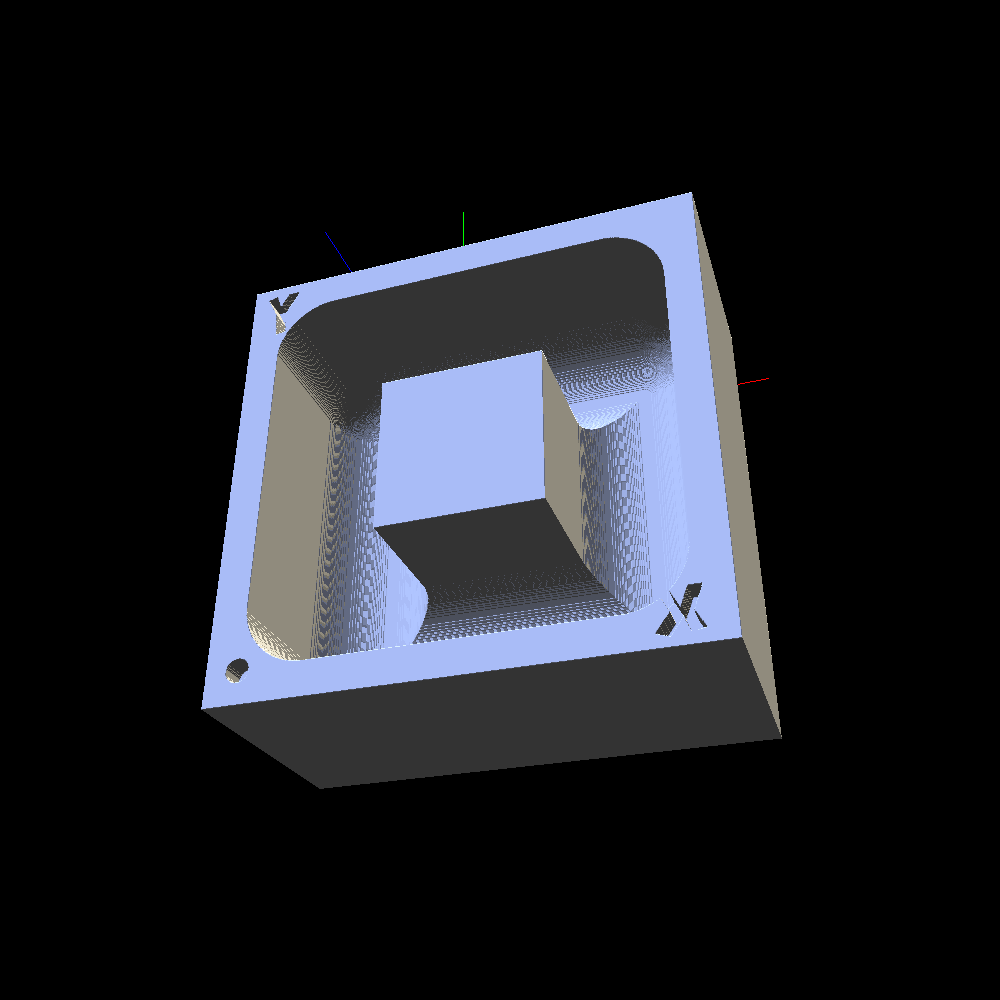
\includegraphics[width=\linewidth]{figures/image16.png} &
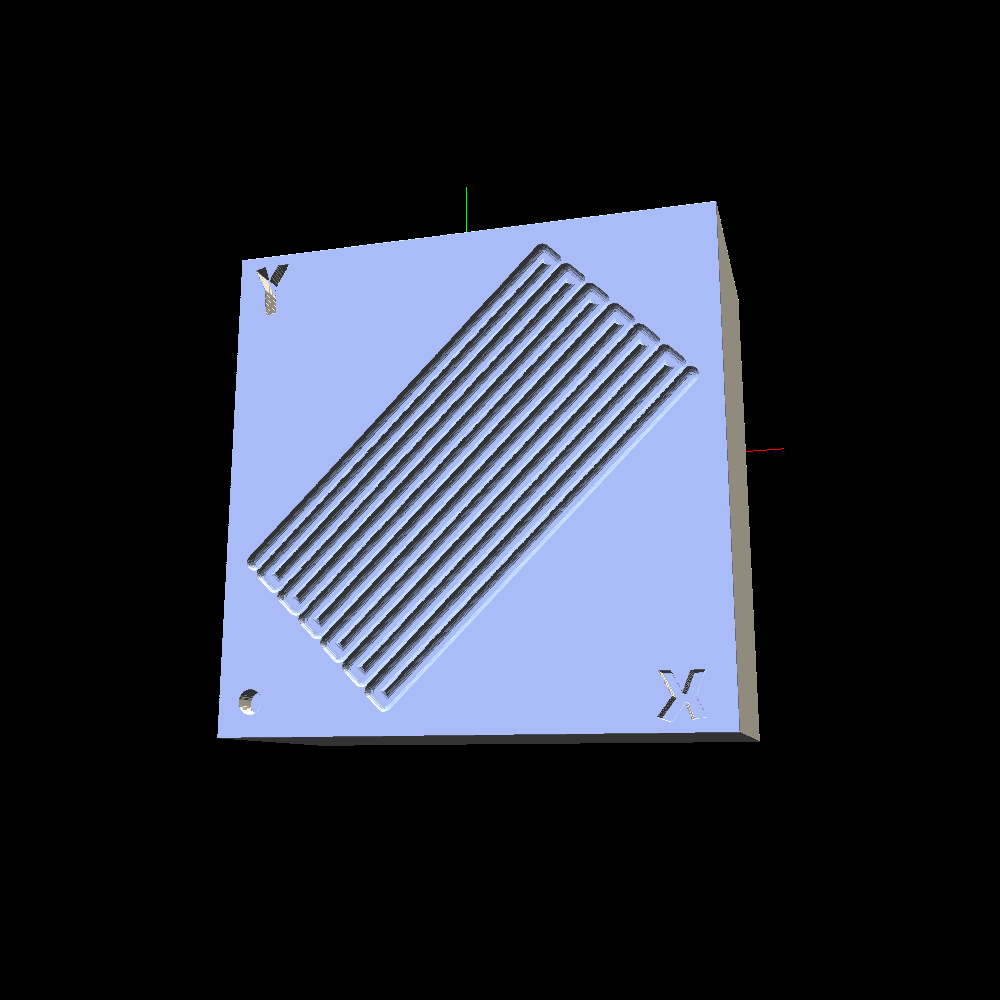
\includegraphics[width=\linewidth]{figures/image17.png} &
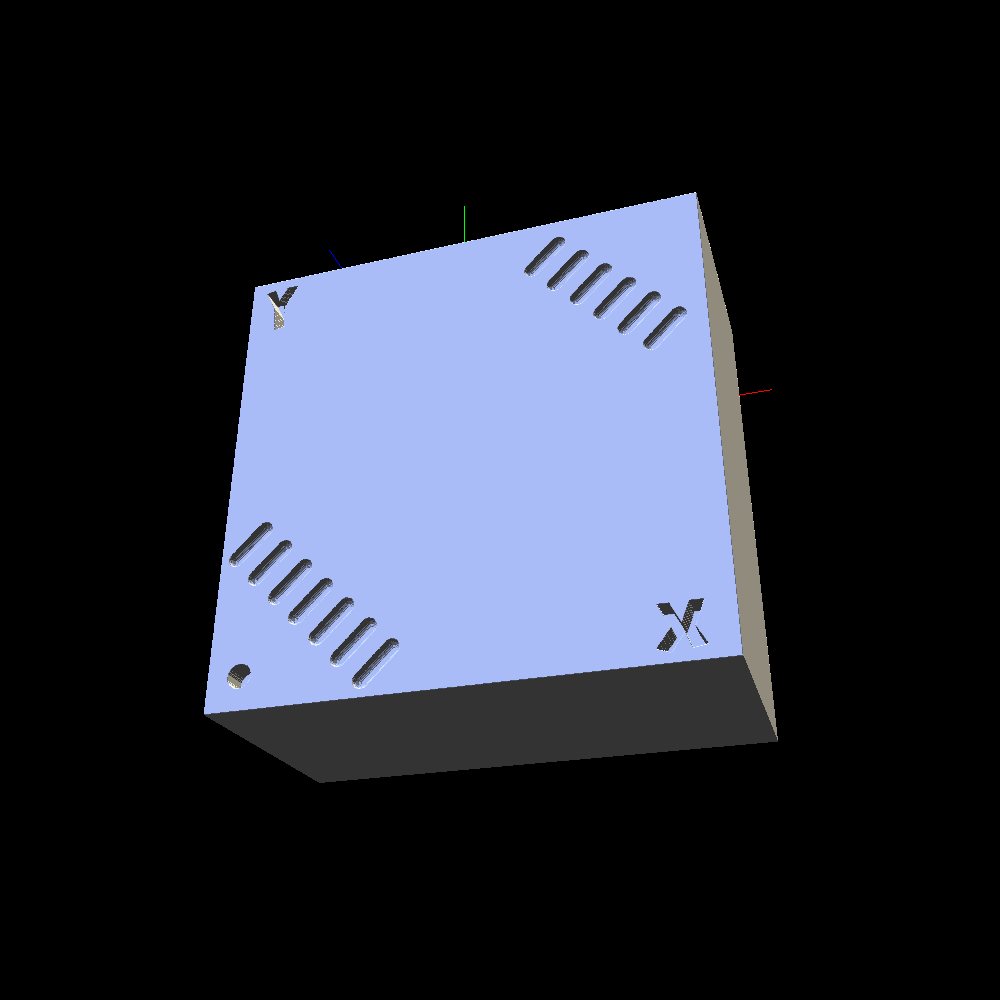
\includegraphics[width=\linewidth]{figures/image18.png} \\
square\_600.gcode & diagonal\_cut.gcode & air\_moves.gcode \\
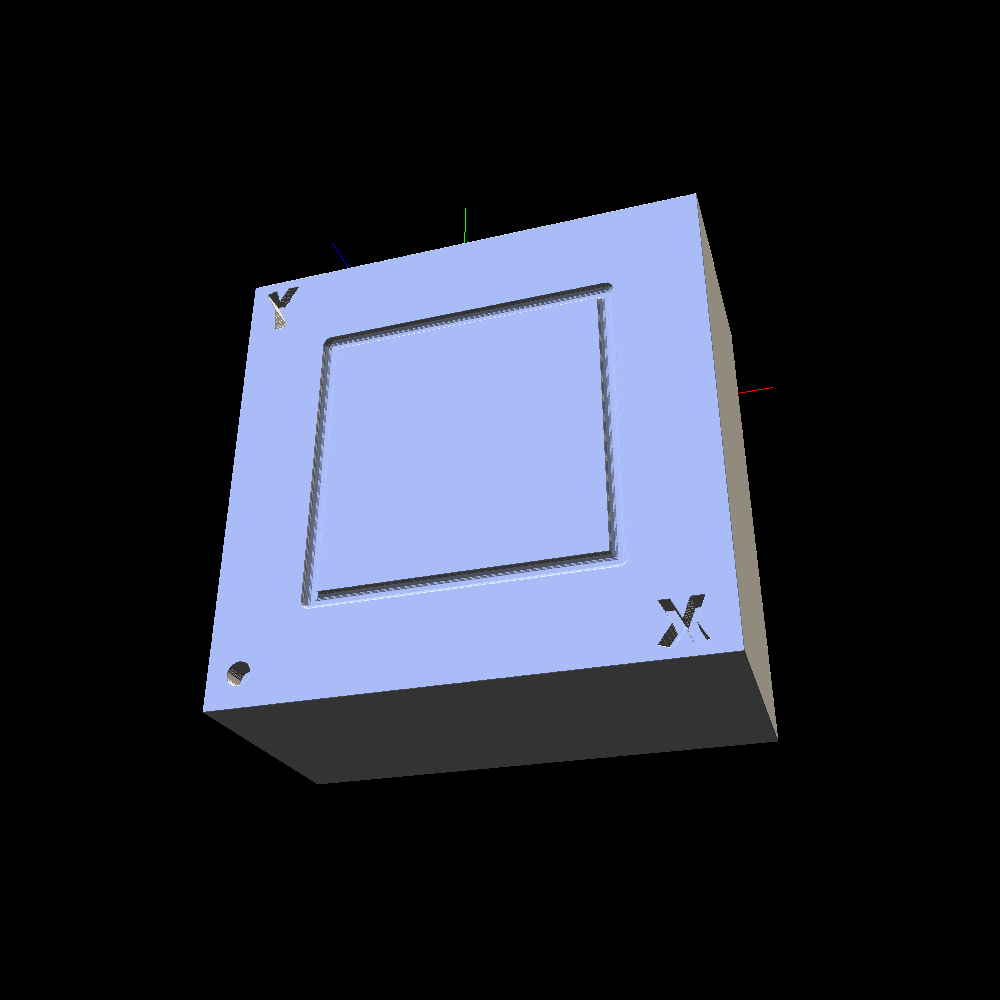
\includegraphics[width=\linewidth]{figures/image19.png}
&
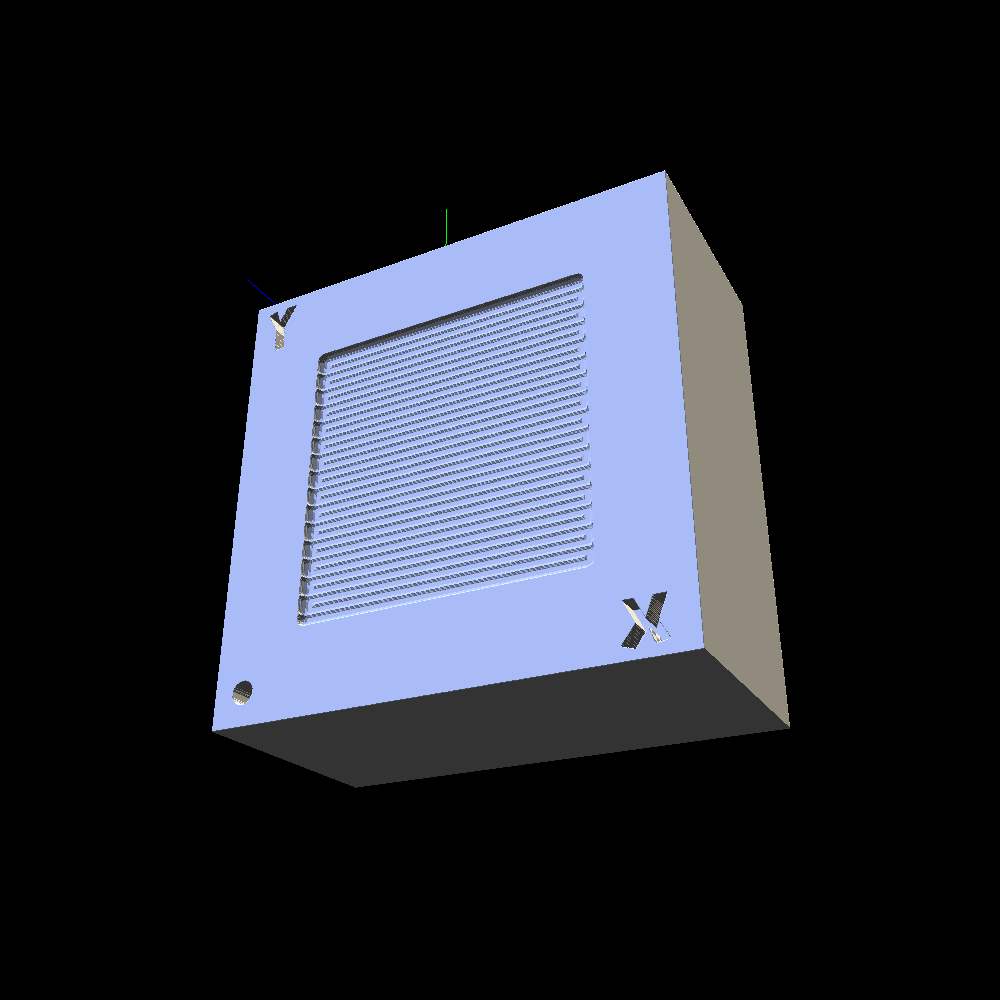
\includegraphics[width=\linewidth]{figures/image20.png}
&
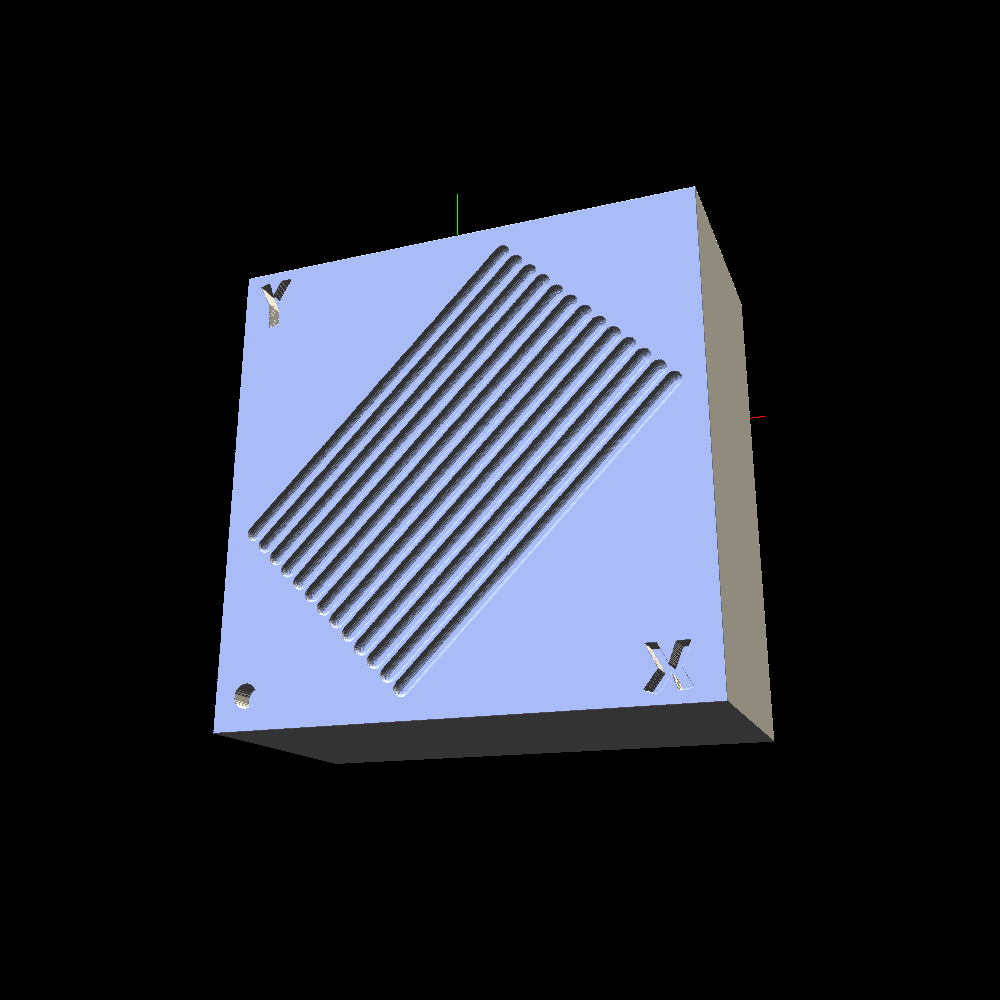
\includegraphics[width=\linewidth]{figures/image21.png} \\
contour.gcode & pocket\_axis.gcode & raster\_45.gcode \\
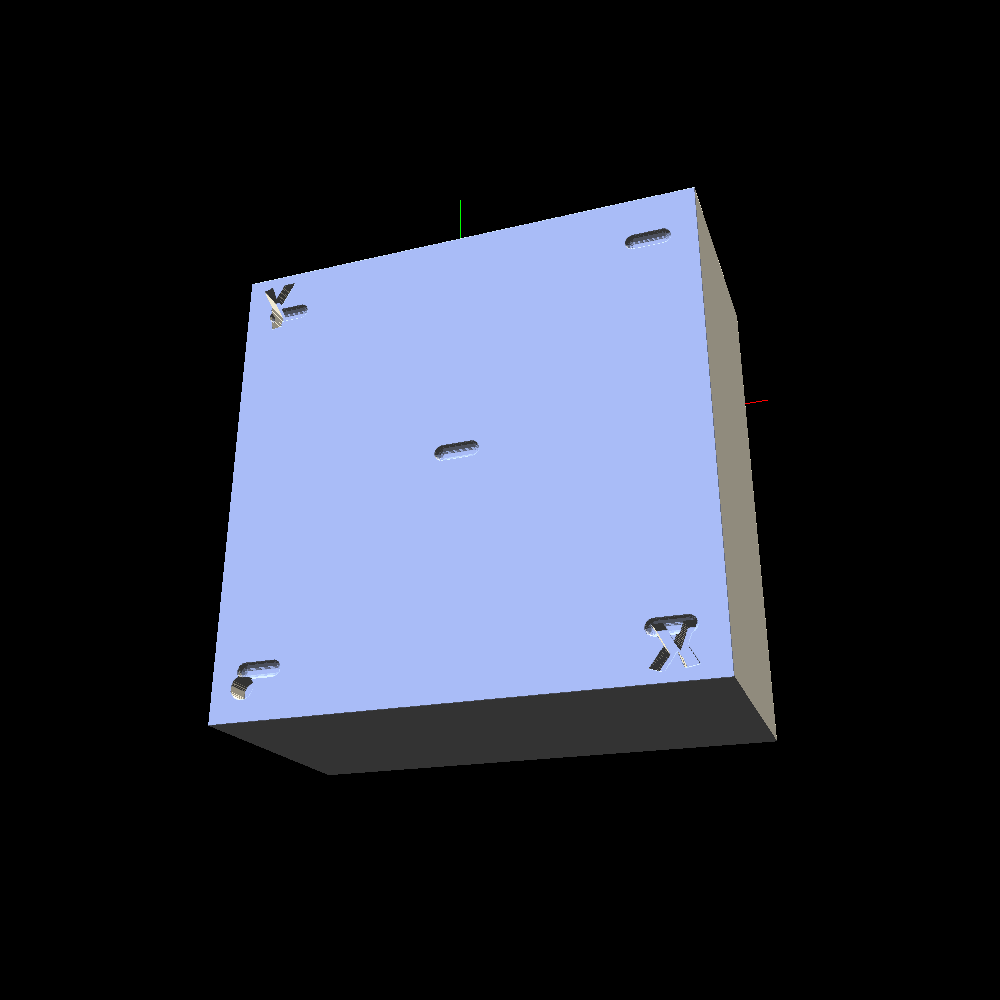
\includegraphics[width=\linewidth]{figures/image22.png}
&
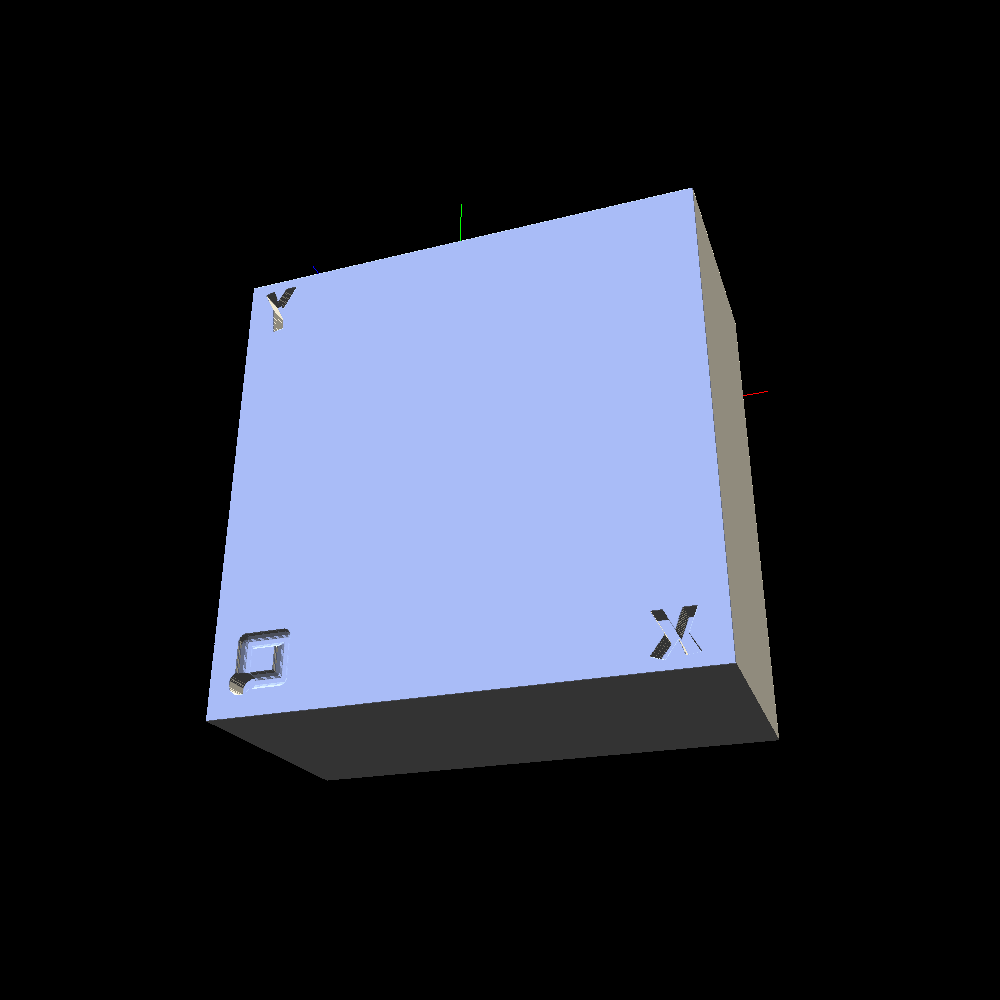
\includegraphics[width=\linewidth]{figures/image23.png}
&
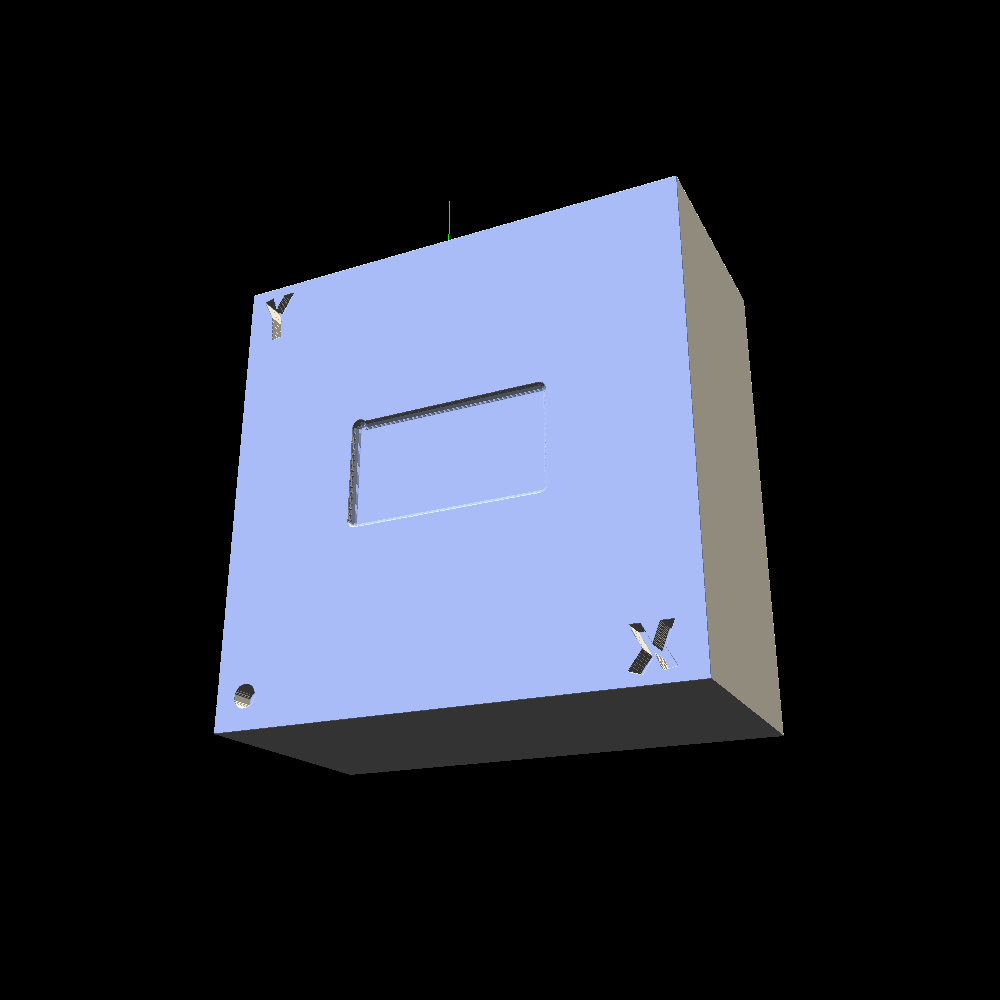
\includegraphics[width=\linewidth]{figures/image24.png} \\
Rapids.gcode & localized.gcode & finishing.gcode \\
\end{longtable}

\hypertarget{references}{%
\subsection{References}\label{references}}

1. T. Van Hook. \emph{Real-time shaded NC milling display.} Computer
Graphics (Proc. SIGGRAPH '86), 20(4):15-20, 1986.

2. H. Müller, T. Surmann, M. Stautner, F. Albersmann, K. Weinert.
\emph{Online sculpting and visualization of multi-dexel volumes.} Proc.
8th ACM Symposium on Solid Modeling and Applications (SM '03), 258-261,
2003.

3. B. Tukora, T. Szalay. \emph{Multi-dexel based material removal
simulation and cutting force prediction with the use of general-purpose
graphics processing units.} Advances in Engineering Software,
43(1):65-70, 2012.

4. M. Inui, M. Kobayashi, N. Umezu. \emph{Cutter engagement feature
extraction using triple-dexel representation workpiece model and GPU
parallel processing.} Computer-Aided Design and Applications,
16(1):89-102, 2019.

5. C. C. L. Wang, Y.-S. Leung, Y. Chen. \emph{Solid modeling of
polyhedral objects by Layered Depth-Normal Images on the GPU.}
Computer-Aided Design, 42(6):535-544, 2010.

6. D. Blackmore, M. C. Leu, L. P. Wang. \emph{The sweep-envelope
differential equation algorithm and its application to NC machining
verification.} Computer-Aided Design, 29(9):629-637, 1997.

7. K. Abdel-Malek, J. Yang, D. Blackmore, K. Joy. \emph{Swept volumes:
foundation, perspectives, and applications.} International Journal of
Shape Modeling, 12(1):87-127, 2006.

8. W. E. Lorensen, H. E. Cline. \emph{Marching cubes: a high resolution
3D surface construction algorithm.} Computer Graphics (Proc. SIGGRAPH
'87), 21(4):163-169, 1987.

9. C. Dyken, G. Ziegler, C. Theobalt, H.-P. Seidel. \emph{High-speed
marching cubes using HistoPyramids.} Computer Graphics Forum,
27(8):2028-2039, 2008.

\textcolor{red}{10. Y. Boz, H. Erdim, I. Lazoglu. \emph{A comparison of solid model and
three-orthogonal dexelfield methods for cutter-workpiece engagement
calculations in three- and five-axis virtual milling.} The International
Journal of Advanced Manufacturing Technology, 81(5-8):811-823, 2015.
\url{https://doi.org/10.1007/s00170-015-7251-7}}

\textcolor{red}{11. Y. Altintas, P. Kersting, D. Biermann, E. Budak, B. Denkena, I.
Lazoglu. \emph{Virtual process systems for part machining operations.}
CIRP Annals, 63(2):585-605, 2014.
\url{https://doi.org/10.1016/j.cirp.2014.05.007}}

\textcolor{red}{12. X. Cao, G. Zhao, W. Xiao. \emph{Digital Twin-oriented real-time
cutting simulation for intelligent computer numerical control
machining.} Proceedings of the Institution of Mechanical Engineers, Part
B: Journal of Engineering Manufacture, 236(1-2):5-15, 2022.
\url{https://doi.org/10.1177/0954405420937869}}

\textcolor{red}{13. H. Erdim, I. Lazoglu, B. Ozturk. \emph{Feedrate scheduling
strategies for free-form surfaces.} International Journal of Machine
Tools and Manufacture, 46(7-8):747-757, 2006.
\url{https://doi.org/10.1016/j.ijmachtools.2005.07.036}}

\textcolor{red}{14. W. Li, B. Li, S. He, X. Mao, C. Qiu, Y. Qiu, X. Tan. \emph{A novel
milling parameter optimization method based on improved deep
reinforcement learning considering machining cost.} Journal of
Manufacturing Processes, 84:1362-1375, 2022.
\url{https://doi.org/10.1016/j.jmapro.2022.11.015}}

\textcolor{red}{15. Y. Zhang, X. Xu, Y. Liu. \emph{Numerical control machining
simulation: a comprehensive survey.} International Journal of Computer
Integrated Manufacturing, 24(7):593-609, 2011.
\url{https://doi.org/10.1080/0951192X.2011.566283}}

\textbf{Declarations}

\textbf{Funding}\\
The authors declare that no funds, grants, or other support were
received during the preparation of this manuscript.

\textbf{Competing interests}

The authors have no relevant financial or non-financial interests to
disclose.

\textbf{Code and data availability}

The simulator, the benchmark G-code programs, the voxelised tool models
and the scripts that reproduce every table in this paper are openly
available at \url{https://github.com/nik71b14/autocam}. The analytic
continuum reference of §4.6 is included as a standalone script with no
dependency on the GPU code path.

\textbf{Author contributions}

{[}to be completed{]}

\end{document}
